\documentclass[a4paper,11pt]{article}

\usepackage[T1]{fontenc}
\usepackage[utf8]{inputenc}
\usepackage{lmodern}
\usepackage{microtype}
\renewcommand{\familydefault}{\sfdefault}

% ------------------------------------------------------------------
% Layout and general packages
% ------------------------------------------------------------------
\usepackage[a4paper,margin=2.5cm]{geometry}
\usepackage[dvipsnames]{xcolor}
\usepackage{graphicx}
\usepackage{enumitem}
\usepackage{booktabs,longtable,array}
\usepackage{amsmath,amssymb}
\usepackage{caption}
\usepackage{listings}
\usepackage[most]{tcolorbox}
\usepackage{tikz}
\usetikzlibrary{arrows.meta,positioning}
\usepackage[colorlinks=true,linkcolor=NavyBlue,urlcolor=NavyBlue,citecolor=NavyBlue]{hyperref}

\setlength{\parindent}{0pt}
\setlength{\parskip}{0.55em}
\setlist{itemsep=2pt,topsep=3pt,parsep=0pt}
\sloppy
\emergencystretch=3em
\captionsetup{font=small,labelfont=bf}

% ------------------------------------------------------------------
% Inline code: \code{...} (no need to escape _ or \ ; avoid # % & and a trailing backslash)
% ------------------------------------------------------------------
\newcommand{\code}[1]{\texttt{\detokenize{#1}}}

% ---- helpers ----
\providecommand{\todo}[1]{\textcolor{red}{[#1]}}
\definecolor{pipeBlue}{HTML}{004C8C}
\definecolor{pipeBg}{HTML}{F4F8FB}
\definecolor{pipeRed}{RGB}{140,0,0}
\definecolor{pipeGreen}{HTML}{355E3B}
\definecolor{swEsc}{HTML}{D96F00}     % ESCON Studio
\definecolor{swIde}{HTML}{00838F}     % Arduino IDE
\definecolor{swPhone}{HTML}{8A3FB5}   % phone / Gobannos
\definecolor{swCode}{HTML}{1F5FBF}    % VS Code terminal (py)
\definecolor{swTerm}{HTML}{4D4D4D}    % Termux / ssh
\newcommand{\swtag}[2]{{\setlength{\fboxsep}{1.8pt}\colorbox{#1}{\textcolor{white}{\scriptsize\textbf{#2}}}}}
\tikzset{
  pstep/.style={draw=pipeBlue,fill=pipeBg,rounded corners=3pt,align=center,text width=3.3cm,
                minimum height=1.6cm,font=\footnotesize,inner sep=3pt},
  pdec/.style={pstep,draw=pipeRed,fill=red!6},
  pok/.style={pstep,draw=pipeGreen,fill=green!8},
  popt/.style={pstep,dashed,fill=white},
  parr/.style={-{Stealth[length=2.2mm]},thick,pipeBlue},
  parrd/.style={-{Stealth[length=2.2mm]},thick,pipeBlue,dashed}
}

% ------------------------------------------------------------------
% Code listings (terminal commands, scripts)
% ------------------------------------------------------------------
\lstdefinestyle{term}{
  basicstyle=\ttfamily\small,
  breaklines=true,
  breakatwhitespace=false,
  postbreak=\mbox{\textcolor{gray}{$\hookrightarrow$}\space},
  columns=fullflexible,
  keepspaces=true,
  upquote=true,
  showstringspaces=false,
  frame=single,
  rulecolor=\color{black!25},
  backgroundcolor=\color{black!3},
  framexleftmargin=3pt,
  xleftmargin=3pt,
  xrightmargin=3pt,
  aboveskip=0.9em,
  belowskip=0.7em,
  captionpos=t
}
\lstset{style=term}

\newtcolorbox{safetybox}[1][Safety]{breakable,enhanced,colback=red!5!white,colframe=red!65!black,
  fonttitle=\bfseries,title=#1,boxrule=0.6pt,arc=2pt}
\newtcolorbox{notebox}[1][Note]{breakable,enhanced,colback=blue!4!white,colframe=blue!55!black,
  fonttitle=\bfseries,title=#1,boxrule=0.6pt,arc=2pt}
\newtcolorbox{okbox}[1][Status]{breakable,enhanced,colback=green!4!white,colframe=green!45!black,
  fonttitle=\bfseries,title=#1,boxrule=0.6pt,arc=2pt}
\newtcolorbox{warnbox}[1][Warning]{breakable,enhanced,colback=orange!6!white,colframe=orange!80!black,
  fonttitle=\bfseries,title=#1,boxrule=0.6pt,arc=2pt}

\newcolumntype{L}[1]{>{\raggedright\arraybackslash}p{#1}}

\title{\textbf{phonefleet + Chipiron}\\[4pt]\large Controlling the motor from laptop + phone (scripts v3)}
\author{Matilde}
\date{\today}

\begin{document}
\maketitle

Current pipeline to run an ESCON motor through Arduino/Python and laptop/phone, with the \textbf{v3} scripts. The full file list and dependencies are in \code{README_chipiron_v3.md}). \textbf{CAUTION:} nothing has been tested on Chipiron itself so far, and \textbf{The LoRa link has not been tested at all} (Section~\ref{sec:limits}). \\

All up-to-date scripts are here: \url{https://github.com/Turbotice/icewave/tree/main/icewave/chipiron}

\begin{notebox}[Setup used]
Windows laptop, VS Code/git, Fairphone (FP4) running the Gobannos app, laptop connected to the phone's Wi-Fi hotspot.
\end{notebox}

\tableofcontents

\newpage

% ==================================================================
\section{Overview and pipeline}
\label{sec:pipeline}
% ==================================================================

\begin{figure}[htbp]
  \centering
  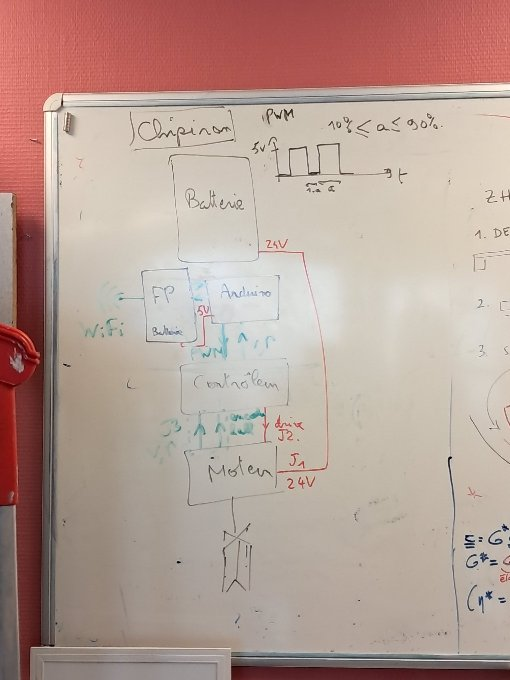
\includegraphics[width=0.85\textwidth]{figures/chipiron_sketch_overview.jpg}%
  \caption{Chipiron overview (sketch by Stéphane)}
  \label{fig:chipiron_overview}
\end{figure}

\begin{figure}[htbp]
  \centering
  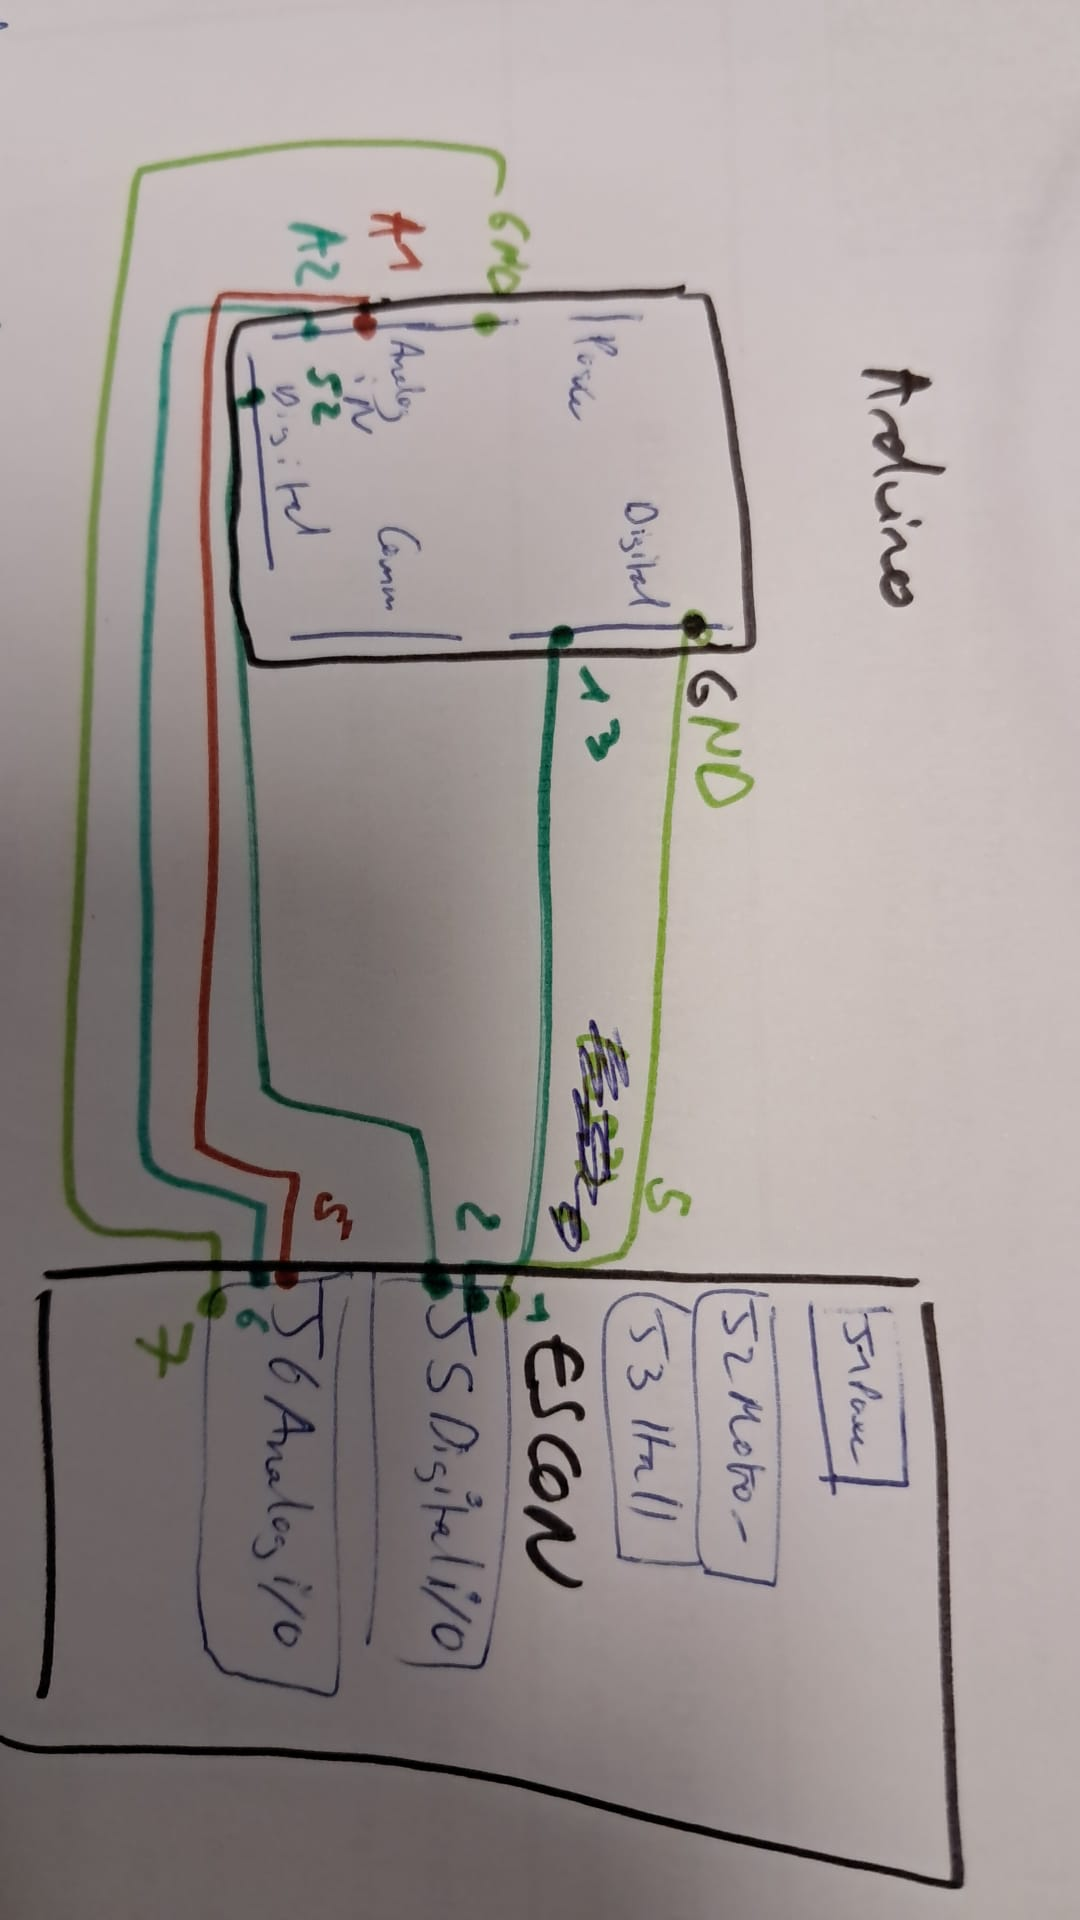
\includegraphics[angle=90, width=0.85\textwidth]{figures/wiring_arduino_escon7010_ECmotor-lab.jpeg}
  \caption{Arduino/ESCON controller plugging (lab EC motor).}
  \label{fig:arduino}
\end{figure}

\textbf{Overall procedure:}
\begin{itemize}
  \item The laptop sends HTTP requests (\code{/start}, \code{http:<phoneIP>:8080/usb-cmd/<command>}, \code{http:<phoneIP>:8080/usb-cmd/e} (enable motor), \code{http:<phoneIP>:8080/usb-cmd/d} (disable motor), \code{/stop}, \code{/status}, \code{/list-files}, \code{/get-file/<name>}).
  \item The \textbf{Gobannos app on the phone} is the HTTP server (port 8080). It forwards \code{<command>} (\code{mo}, \code{c60.0}, \code{o50,20,0.2}, \code{x}, \code{e}, \code{d}\ldots) to the Arduino over USB, records the sensors of the phone and logs the bytes sent back by the Arduino (the ``Usb'' file).
  \item The \code{PWM_full_v3.ino} firmware is flashed on the \textbf{Arduino Mega} from the Arduino IDE on a laptop (board \emph{Arduino Mega 2560}), only once before running experiments. It outputs a PWM duty cycle on pin 13 (ESCON set value), drives the enable line (pin 52) and sends back two analog readings (A1, A2) every 250\,ms.
  \item The \textbf{ESCON 70/10} turns the duty cycle into a speed set value using the mapping stored in its \code{.edc} parameters. The \emph{same} \code{.edc} file is read by the Python scripts, so that rpm $\leftrightarrow$ duty conversions, the rest duty (duty that gives 0\,rpm) and the ESCON speed ramp limits are always those of the controller.
\end{itemize}

Below: step-by-step route for one test. Termux is \textbf{not} used for the experiment (Gobannos only); it is kept for diagnosis (Section~\ref{sec:ssh}). Optional steps (parameter patching, ramp planning, manual checks, clock synchronisation, offline decoding) are shown dashed in Figure~\ref{fig:pipeline} and described in the subsection with the same number or in the one indicated.

\begin{figure}[htbp]
\centering
\resizebox{\textwidth}{!}{%
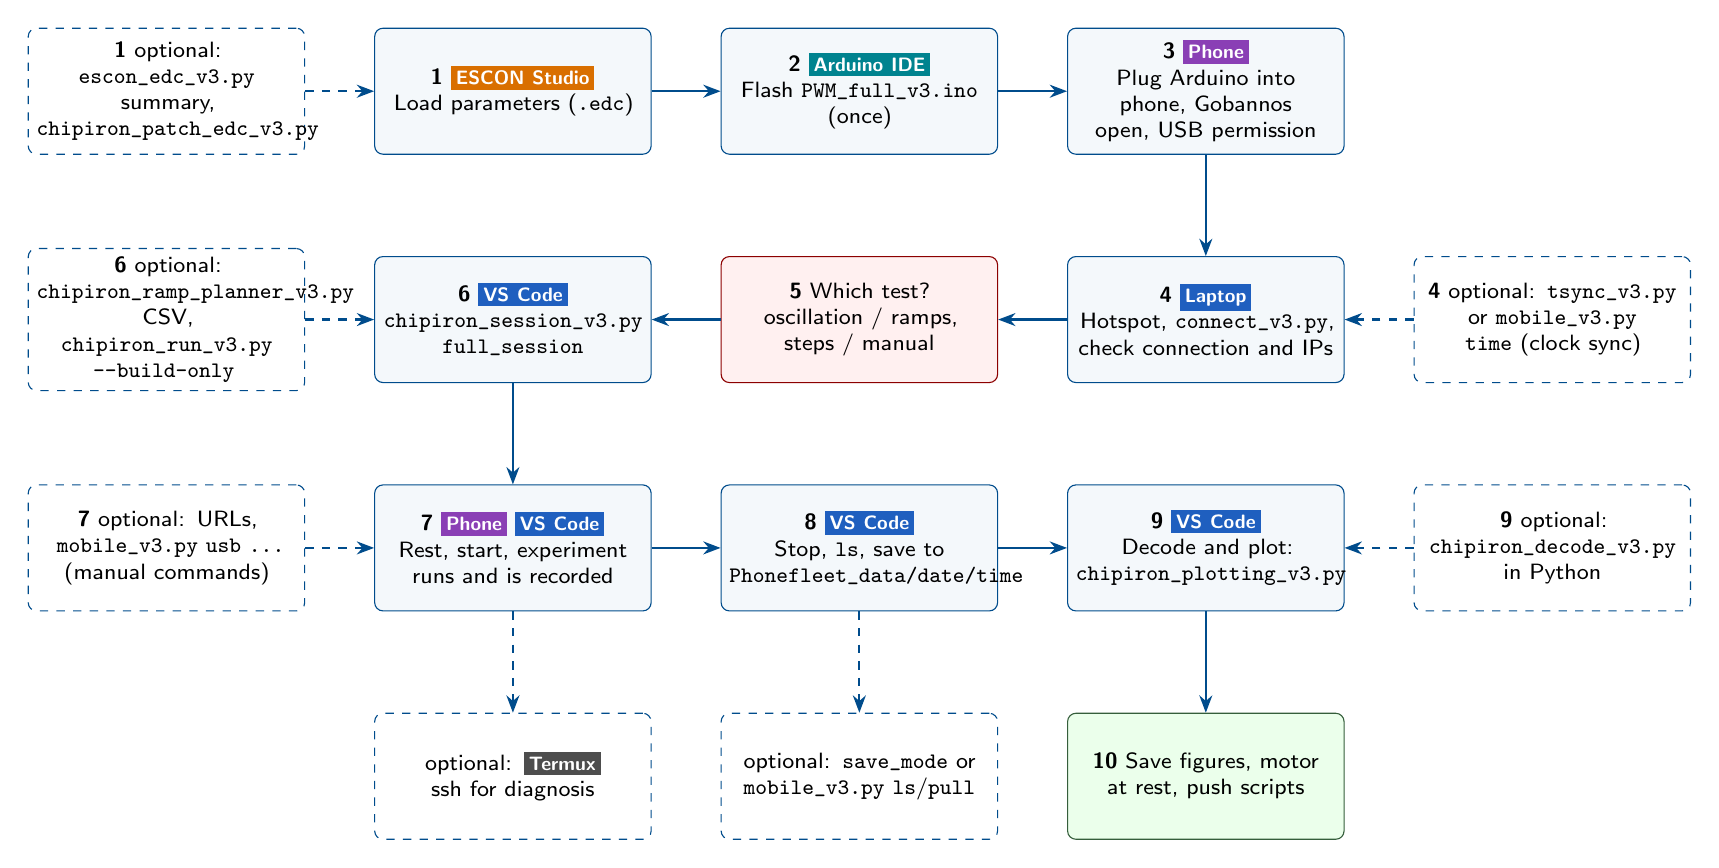
\begin{tikzpicture}
% ---- main chain (numbers = subsections of this section)
\node[pstep] (n1) at (0,0) {\textbf{1} \swtag{swEsc}{ESCON Studio}\\ Load parameters (\code{.edc})};
\node[pstep] (n2) at (4.4,0) {\textbf{2} \swtag{swIde}{Arduino IDE}\\ Flash \code{PWM_full_v3.ino} (once)};
\node[pstep] (n3) at (8.8,0) {\textbf{3} \swtag{swPhone}{Phone}\\ Plug Arduino into phone, Gobannos open, USB permission};

\node[pstep] (n6) at (0,-2.9) {\textbf{6} \swtag{swCode}{VS Code}\\ \code{chipiron_session_v3.py}\\ \code{full_session}};
\node[pdec]  (n5) at (4.4,-2.9) {\textbf{5} Which test?\\ oscillation / ramps, steps / manual};
\node[pstep] (n4) at (8.8,-2.9) {\textbf{4} \swtag{swCode}{Laptop}\\ Hotspot, \code{connect_v3.py}, check connection and IPs};

\node[pstep] (n7) at (0,-5.8) {\textbf{7} \swtag{swPhone}{Phone}\ \swtag{swCode}{VS Code}\\ Rest, start, experiment runs and is recorded};
\node[pstep] (n8) at (4.4,-5.8) {\textbf{8} \swtag{swCode}{VS Code}\\ Stop, \code{ls}, save to \code{Phonefleet_data/date/time}};
\node[pstep] (n9) at (8.8,-5.8) {\textbf{9} \swtag{swCode}{VS Code}\\ Decode and plot: \code{chipiron_plotting_v3.py}};

\node[pok]   (n10) at (8.8,-8.7) {\textbf{10} Save figures, motor at rest, push scripts};
\node[popt]  (o1) at (4.4,-8.7) {optional: \code{save_mode} or \code{mobile_v3.py} \code{ls}/\code{pull}};
\node[popt]  (o2) at (0,-8.7) {optional: \swtag{swTerm}{Termux} ssh for diagnosis};

% ---- optional tools
\node[popt] (oA) at (-4.4,0) {\textbf{1} optional: \code{escon_edc_v3.py} summary, \code{chipiron_patch_edc_v3.py}};
\node[popt] (oB) at (-4.4,-2.9) {\textbf{6} optional: \code{chipiron_ramp_planner_v3.py} CSV, \code{chipiron_run_v3.py --build-only}};
\node[popt] (oC) at (-4.4,-5.8) {\textbf{7} optional: URLs, \code{mobile_v3.py} \code{usb ...} (manual commands)};
\node[popt] (oD) at (13.2,-2.9) {\textbf{4} optional: \code{tsync_v3.py} or \code{mobile_v3.py} \code{time} (clock sync)};
\node[popt] (oE) at (13.2,-5.8) {\textbf{9} optional: \code{chipiron_decode_v3.py} in Python};

\draw[parr] (n1)--(n2);
\draw[parr] (n2)--(n3);
\draw[parr] (n3)--(n4);
\draw[parr] (n4)--(n5);
\draw[parr] (n5)--(n6);
\draw[parr] (n6)--(n7);
\draw[parr] (n7)--(n8);
\draw[parr] (n8)--(n9);
\draw[parr] (n9)--(n10);
\draw[parrd] (n8)--(o1);
\draw[parrd] (n7)--(o2);
\draw[parrd] (oA)--(n1);
\draw[parrd] (oB)--(n6);
\draw[parrd] (oC)--(n7);
\draw[parrd] (oD)--(n4);
\draw[parrd] (oE)--(n9);
\end{tikzpicture}}
\caption{Pipeline of one Chipiron test. Dashed boxes are optional or for quick tests and debugging. The numbers match the subsections of this section.}
\label{fig:pipeline}
\end{figure}

\newpage
% ------------------------------------------------------------------
\subsection{ESCON Studio: load the parameters}\label{sec:pipe-escon}
% ------------------------------------------------------------------
\swtag{swEsc}{ESCON Studio}\ \swtag{swCode}{VS Code}\ (optional tools: \code{escon_edc_v3.py}, \code{chipiron_patch_edc_v3.py})

\begin{itemize}
  \item \textbf{Read} an \code{.edc} before loading it: \code{escon_edc_v3.py} prints the motor type, operation mode, PWM mapping (value at 10, 50 and 90\,\%, duty giving 0\,rpm, polarity), speed ramp, and the analog-output conversion (volts $\rightarrow$ rpm and A). It also warns about inconsistencies (for instance an offset adjust stored but not enabled). The same file is read by every script (session, run, oscillate, planner, plotting).
  \item \textbf{Edit} (a copy of) an \code{.edc} with \code{chipiron_patch_edc_v3.py}: analog-output shift to 0--4\,V, bipolar set value, speed ramp, motor type, offset.  Always \textbf{open the result in ESCON Studio and check every value} before writing it to the controller.
  \item Keep the controller \textbf{disabled} while loading the \code{.edc}; double-check every parameter in the software and edit by hand if required.
  \item The ESCON configuration must match the Arduino mode of the test (Section~\ref{sec:pipe-choice}): \textbf{bipolar} (\code{mo}: 10\,\%~$\rightarrow -800$\,rpm, 50\,\%~$=0$\,rpm, 90\,\%~$\rightarrow +800$\,rpm) or \textbf{unipolar} (\code{mc}: 10\,\%~$\rightarrow 0$\,rpm, 90\,\%~$\rightarrow 800$\,rpm). With a bipolar \code{.edc}, ramps and steps run in \code{mo} too (\code{c<duty>} is accepted in both modes).
  \item Optional: keep the real-time speed/current display visible in ESCON Studio (\textit{Tools > Data recorder > right click on graph to export data}; only the current time window is exported).
\end{itemize}

\begin{lstlisting}[title={Terminal (VS Code): read an .edc}]
py escon_edc_v3.py parameters_Sep26.edc --folder edc_summaries
py escon_edc_v3.py parameters_Sep26.edc --no-save
py escon_edc_v3.py
\end{lstlisting}
The first line prints the summary and saves it as \code{.txt} in \code{edc_summaries}; the second prints only; the third asks for the file and whether to save.

\begin{lstlisting}[title={Terminal (VS Code): build a patched copy}]
py chipiron_patch_edc_v3.py --in parameters_Sep26.edc --out parameters_Sep26_v2.edc --bipolar-setpoint 800 --ramp 2000 --motor-type DC --offset -11
\end{lstlisting}

\begin{longtable}{@{}L{4.6cm}L{10.4cm}@{}}
\toprule
\textbf{Argument} & \textbf{Meaning} \\
\midrule
\endhead
\code{--in FILE}, \code{--out FILE} & source \code{.edc} and the \emph{new} file (must not exist, unless \code{--force}; must differ from \code{--in}) \\
\code{--ao-shift} / \code{--no-ao-shift} & remap the two analog outputs to 0--4\,V so that the Arduino (0--5\,V ADC) can read negative values: speed $-1000\ldots+1000$\,rpm $\rightarrow$ 0--4\,V, current $-5\ldots+5$\,A $\rightarrow$ 0--4\,V. \textbf{On by default and required with the bipolar mapping} (see the box below). Use \code{--no-ao-shift} only if the file already has the shift (e.g.\ a file whose name ends in \code{_ao_shift}) \\
\code{--speed-range R}, \code{--current-range I} & rpm and A at full scale of the AO shift (defaults 1000 and 5) \\
\code{--bipolar-setpoint R} & PWM set value becomes bipolar: 10\,\% $=-R$, 50\,\% $=0$, 90\,\% $=+R$ rpm \\
\code{--ramp RPM_PER_S} & ESCON speed ramp (acceleration and deceleration) \\
\code{--motor-type EC|DC} & written \emph{only} when given. Enum of the \code{.edc}: 0 = EC (brushless), 1 = DC (brushed); a wrong value can make the controller drive the motor wrongly \\
\code{--offset RPM} & fixed set-value offset (can be negative). It only acts if the offset functionality is \emph{enabled} in ESCON Studio; the script prints the state of the enable bit \\
\code{  --speed-p-gain N } &   speed controller P gain (integer, no unit, as shown in ESCON Studio). Written to the regulator actually in use: Speed 1 (mode of controller "Current Limiter") or Speed 2 ("Inner Current Control Loop"); the script says which one. Too low a gain flattens /skews fast sines; too high gives noise or oscillation: raise it step by step \\
\code{--force} & overwrite \code{--out} \\
\bottomrule
\end{longtable}

    .

\begin{notebox}[Bipolar mapping $\Rightarrow$ use the AO shift]
With bipolar PWM mapping the motor reverses, so the actual speed and current become negative. The analog outputs of \code{parameters_Sep26.edc} as delivered are \emph{not} shifted ($\pm4$\,V around 0\,V): a negative speed would be a negative voltage on the Arduino pin, which reads it as 0 (and a pin pushed below about $-0.5$\,V is outside the ATmega ratings). The AO shift (default of the patch script) maps the outputs to 0--4\,V with 0\,rpm and 0\,A at 2\,V:
\[
  \text{speed}=\frac{V-2}{0.002}\ \text{rpm}\ (\pm1000\,\text{rpm range}),\qquad
  \text{current}=\frac{V-2}{0.4}\ \text{A}\ (\pm5\,\text{A range}),\qquad V=\text{adc}\cdot V_{\mathrm{ref}}/1023 .
\]
 Choose \code{--speed-range} at least as large as the maximum speed: 4\,V corresponds to $+$range (the ADC still reads up to 5\,V, i.e.\ 1.25 times the range, then saturates) and one ADC count is $\approx0.0024\times\text{range}$\,rpm (2.4\,rpm for 1000\,rpm, about 6\,rpm for the 2460\,rpm of the Chipiron configuration). \textbf{Which AO feeds which Arduino pin is hardware} (AO1 $\rightarrow$ A1, AO2 $\rightarrow$ A2, current on AO1 and speed on AO2 in the lab, Section~\ref{sec:a1a2}); \textbf{which quantity each AO outputs is set in the \code{.edc}} (\code{PARAM_AnalogOutputsConfiguration}, here AO1 = Actual Current, AO2 = Actual Speed). 
\end{notebox}

\begin{notebox}[Procedure: offset]
The offset should be tuned so that the rest command (\code{c50.0} in bipolar mapping) gives nearly 0\,rpm. Tune it by hand in ESCON Studio (send \code{c50.0} and check the speed), then use \code{chipiron_patch_edc_v3.py --offset} to store it, \textbf{and check that the offset adjust is enabled} in ESCON Studio. 
\end{notebox}


\begin{notebox}[Debugging and warnings]
If in ESCON Studio the ``PWM value'' is stuck at an out-of-range value and the motor is stuck in disabled/error mode, check that the Arduino is actually plugged in and running (a reset Arduino now boots with the motor disabled until it receives \code{mo}, \code{mc} or \code{e}).
\end{notebox}

% ------------------------------------------------------------------
\subsection{Arduino IDE: flash \texttt{PWM\_full\_v3.ino}}\label{sec:pipe-ino}
% ------------------------------------------------------------------
\swtag{swIde}{Arduino IDE} Board \emph{Arduino Mega 2560}, flashed from the laptop \textbf{once}; afterwards unplug it from the laptop and plug it into the phone.  Two running modes are chosen at run time by a text command.

\begin{longtable}{@{}L{4.4cm}L{2.6cm}L{8.0cm}@{}}
\toprule
\textbf{Command} & \textbf{Mode} & \textbf{Effect} \\
\midrule
\endhead
\code{mc} & constant & select constant mode (rest duty 10\,\%), go to rest, \textbf{enable the motor} \\
\code{mo} & oscillation & select oscillation mode (rest duty 50\,\%), go to rest, \textbf{enable the motor} \\
\code{c<duty>} & both & constant duty in \%, decimals accepted: \code{c50}, \code{c60.5} \\
\code{o<mean>,<amp>,<freq>} & oscillation only & sine on the duty: \code{o50,20,0.5} = 50\,\% $\pm 20$\,\% at 0.5\,Hz; the Arduino builds the sine at 100\,Hz, starting at the mean going up \\
\code{x} & both & back to the rest duty of the current mode \\
\code{e} & both & enable the ESCON (enable line high) \\
\code{d} & both & rest duty, then disable the ESCON: motor coasts, \emph{no braking} (send \code{x} and wait first for a controlled stop) \\
\bottomrule
\end{longtable}

\begin{itemize}
  \item \textbf{Safe start (new):} at power-up or reset the motor is \emph{disabled} (switch \code{START_ENABLED 0}) and the default mode is oscillation (bipolar, current \code{.edc}). Before, the Arduino booted in constant mode with the motor enabled: with a bipolar \code{.edc} the 10\,\% rest duty means full negative speed until a mode was sent.
  \item Switches at the top of the file: \code{DEFAULT_MODE}, \code{START_ENABLED}, \code{REST_DUTY_CONST} (10), \code{REST_DUTY_OSC} (50), \code{USE_LORA} (0, \textbf{untested}).
  \item The Arduino \textbf{resets} every time it is re-plugged or its USB port is re-opened: send the mode again at each session (the session script does it).
  \item Telemetry: 4 bytes every 250\,ms (details in Section~\ref{sec:pipe-plot}). 
\end{itemize}


% ------------------------------------------------------------------
\subsection{Phone: plug the Arduino, Gobannos, hotspot}\label{sec:pipe-phone}
% ------------------------------------------------------------------
\swtag{swPhone}{Phone}

\begin{enumerate}
  \item Hotspot on, Gobannos open in the foreground; note the IP it shows (Section~\ref{sec:pipe-laptop}).
  \item Plug the Arduino into the phone and accept the USB permission for \textbf{Gobannos}. Do not mix with a Serial USB terminal app.
\end{enumerate}

% ------------------------------------------------------------------
\subsection{Laptop: connection and IP settings}\label{sec:pipe-laptop}
% ------------------------------------------------------------------
\swtag{swCode}{VS Code}\ \swtag{swTerm}{PowerShell}

\begin{itemize}
  \item Connect the laptop to the phone's hotspot.
  \item \code{connect_v3.py}: \code{IP_PREFIX}, \code{NETWORK}, \code{DEFAULT_PHONELIST} (with \code{IP_PREFIX = "10"}, phone 36 is \code{10.153.247.36}). The session asks for phone ID and network number (defaults from this file) and gives the resulting IP to every script it launches. \code{py connect_v3.py} prints the configured addresses and scans the subnet with \code{nmap} (must be installed).
  \item Python packages: \code{ numpy pandas matplotlib} (\code{pyserial} only for LoRa). 
\end{itemize}

To check the laptop/phone connection:
\begin{lstlisting}[title={PowerShell (laptop)}]
ping <phone-ip>
Test-NetConnection -ComputerName <phone-ip> -Port 8080
\end{lstlisting}
\emph{Expected result:} 4 successful replies with \texttt{0\% loss}, and \code{TcpTestSucceeded : True}. If requests time out, confirm your laptop is connected to the phone's active hotspot, and that Gobannos is open in the foreground.

Browser check: \code{http://<phone-ip>:8080/status} should show \code{STOPPED} (or a running state). \\


Clone repository with all my scripts: \url{https://github.com/Turbotice/icewave/tree/main/icewave/chipiron}

\textbf{Install phonefleet }
This is no longer needed for v3 of my scripts, but it is required for termux/ssh debugging. 

\begin{enumerate}
  \item Clone \code{phonefleet} (https://github.com/Turbotice/phonefleet) in VS Code. 
  \item In the terminal, in the folder that contains \code{setup.py}: \code{pip install -e .}
  \item Check: \code{py -c "import phonefleet.server.connect as c; print(c.__file__)"}. If you get \code{ModuleNotFoundError}, the likely causes are a different Python environment than the one used for \code{pip install -e .}, or missing \code{__init__.py} files in the \code{phonefleet/} subfolders.
\end{enumerate}

\paragraph{Find the phone's IP.}\label{sec:ip} Any of these:
\begin{itemize}
  \item \textbf{Gobannos app (easiest)}: it displays the IP when started.
  \item \textbf{Termux} (needs \code{pkg install termux-api} and the Termux:API app): \code{termux-wifi-connectioninfo}; the \code{"ip"} field is the phone's address. This worked.
  \item \textbf{Laptop}, with the hotspot connected: \code{ipconfig} (PowerShell), then in the Wi-Fi section the \textbf{default gateway} (``Passerelle par d\'efaut'') is the phone's IP.
\end{itemize}

\paragraph{USB access.}\label{sec:usb} In Gobannos, if the \textbf{USB STATUS} line first shows \emph{``demande de permission USB non envoy\'ee''}, the phone cannot talk to the Arduino (\code{/usb-cmd/...}).
\begin{enumerate}
  \item Plug the Arduino into the phone (USB cable / OTG adapter).
  \item Accept the Android permission pop-up for the USB device and choose Gobannos.
  \item Check in Gobannos that the USB status changed, and send some URL commands to see that communication is established (Section~\ref{sec:firsttest}).
\end{enumerate}

% ------------------------------------------------------------------
\subsection{Which test?}\label{sec:pipe-choice}
% ------------------------------------------------------------------

\begin{longtable}{@{}L{3.1cm}L{1.9cm}L{2.8cm}L{4.6cm}L{2.2cm}@{}}
\toprule
\textbf{Test} & \textbf{Arduino mode} & \textbf{ESCON mapping} & \textbf{Script run by the session} & \textbf{Rest duty}\\
\midrule
\endhead
Oscillation, firmware mode (smooth sine) & \code{mo} & bipolar & \code{chipiron_oscillate_v3.py --mode firmware} & 50\,\% \\
\addlinespace
Oscillation, stream mode (coarse, not recommended) & \code{mo} or \code{mc} & bipolar or unipolar & \code{chipiron_oscillate_v3.py --mode stream} & from \code{.edc} \\
\addlinespace
Constant speed, ramps, steps, up/down cycles, ramp-planner CSV & \code{mo} (bipolar) or \code{mc} (unipolar) & bipolar or unipolar & \code{chipiron_run_v3.py} & from \code{.edc} \\
\addlinespace
Manual (URL/keyboard commands, any other script) & any & any & none or your script & from \code{.edc} \\
\bottomrule
\end{longtable}

\begin{safetybox}[Motor mapping and test types]
The rest duty of the Arduino mode (\code{mc} 10\,\%, \code{mo} 50\,\%) must give 0\,rpm with the \code{.edc} loaded in ESCON Studio. \code{chipiron_session_v3.py} stops with an ERROR if they do not match, and refuses firmware-mode oscillation with \code{mc} or with a unipolar \code{.edc}. 
\end{safetybox}

% ------------------------------------------------------------------
\subsection{Run the session: \texttt{chipiron\_session\_v3.py}}\label{sec:pipe-session}
% ------------------------------------------------------------------
\swtag{swCode}{VS Code} terminal, with \code{connect_v3.py}, \code{run_gobannos_v3.py}, \code{escon_edc_v3.py}, \code{chipiron_helpers_v3.py}, \code{chipiron_run_v3.py} and \code{chipiron_oscillate_v3.py} next to the script (\code{mobile_v3.py} is not needed, only optional).

\subsubsection{Launch and sequence}

\begin{lstlisting}[title={Terminal (VS Code)}]
py chipiron_session_v3.py                                   (asks the mode)
py chipiron_session_v3.py save_mode                         (no experiment: ls, save )
py chipiron_session_v3.py full_session                      (asks Arduino mode, .edc)
py chipiron_session_v3.py full_session mo                   (bipolar: oscill, ramps, steps)
py chipiron_session_v3.py full_session mc                   (unipolar: ramps, steps)
py chipiron_session_v3.py full_session mo parameters_Sep26.edc
py chipiron_session_v3.py full_session skip                 (send no mode)
\end{lstlisting}
The \code{.edc} can be anywhere on the line; without it the script asks (default = the one used last). \code{skip} leaves the Arduino as is: after a reset the motor stays \emph{disabled} until you send \code{e}, \code{mo} or \code{mc}.

Sequence of a \code{full_session}:
\begin{enumerate}
  \item phone ID and network number $\rightarrow$ IP; the \code{.edc} is loaded \textbf{once} (summary printed) and handed to every script launched afterwards (environment variables), so none of them asks for it again;
  \item status of the phone;
  \item Arduino mode \code{mc}/\code{mo}/\code{skip}: checked against the \code{.edc}, then sent (this also enables the motor at the rest duty);
  \item choice of experiment and \textbf{all its questions}, asked \emph{before} the acquisition starts (errors such as a duty out of range stop the session here, nothing has moved);
  \item 0\,rpm command (\code{c<rest duty>} computed from the \code{.edc}: \code{c50.0} bipolar, \code{c10.0} unipolar), then a wait of \code{ZERO_WAIT_S} = 30\,s at rest;
  \item \code{/start} (acquisition on the phone), experiment runs (scripts are called with \code{--no-record}, so they do not call \code{/start} and \code{/stop});
  \item motor sent back to rest in any case (also on Ctrl-C), \code{/stop}, \code{ls}, save.
\end{enumerate}


\subsubsection{Choice 1: manual}\label{sec:s-manual}
The acquisition starts, then the script waits. Type at the \code{>} prompt: \code{e} (enable), \code{d} (disable), \code{x} (rest), \code{c60.0} (duty), \code{o50,20,0.2} (sine, \code{mo} only); \textbf{Enter stops} the acquisition. The motor is sent back to rest afterwards. Useful to test the chain, or for the A1/A2 identification (Section~\ref{sec:firsttest}).

\subsubsection{Choice 2: oscillation (firmware or stream)}\label{sec:osc-run}

\begin{longtable}{@{}L{4.6cm}L{2.5cm}L{7.9cm}@{}}
\toprule
\textbf{Prompt} & \textbf{Example} & \textbf{Meaning} \\
\midrule
\endhead
Oscillation mode & \code{firmware} & \code{firmware}: one message \code{o<mean>,<amp>,<freq>}, the Arduino builds the sine at 100\,Hz (needs \code{mo} and a bipolar \code{.edc}); default when these hold. \code{stream}: Python sends a new \code{c<duty>} every \code{--dt} s, works with anything but is coarse and \textbf{not recommended} (steps of 0.1\,\% duty, only for periods $\gtrsim 20$\,s, less smooth sines) \\
Mean speed (rpm) & \code{0} & \code{--mean-rpm}; 0 = oscillate around standstill (bipolar); default 400 if unipolar \\
Amplitude (rpm) & \code{100} & \code{--amp-rpm}; below about 80\,rpm ($\pm4$\,\% duty) the sign did not reverse on the lab motor (Section~\ref{sec:osc}) \\
Frequency (Hz) & \code{0.1} & \code{--freq} \\
Number of cycles & \code{5} & \code{--cycles}; duration = cycles / frequency (50\,s here) \\
Extra arguments & Enter & optional: \code{--song}, \code{--dt 0.5} (stream), \code{--verbose} \\
\bottomrule
\end{longtable}

The session already checks (before starting): mean $\pm$ amplitude must fit in 10--90\,\% duty, and the \emph{peak acceleration} of the sine, $\text{amp}\cdot 2\pi f$, is compared with the ESCON speed ramp (2000\,rpm/s here): above it the limiter flattens the sine, a warning gives the largest usable amplitude and asks for confirmation. The rpm are converted with the \code{.edc} mapping (duty amplitude = amp\,/\,20\,rpm per \%). With these values, \code{chipiron_oscillate_v3.py} sends one message, \code{o50.00,5.00,0.1000}, and the firmware builds the sine. The script can also be run alone (\code{--no-record} when the acquisition is handled elsewhere; \code{--yes} skips the confirmation):


\begin{lstlisting}[title={Terminal (VS Code): oscillation examples}]
py chipiron_oscillate_v3.py --edc parameters_Sep26.edc --mean-rpm 0 --amp-rpm 100 --freq 0.1 --cycles 5
py chipiron_oscillate_v3.py --mean-rpm 0 --amp-rpm 300 --freq 0.5 --cycles 10 --no-record --yes
py chipiron_oscillate_v3.py --mode stream --dt 1 --mean-rpm 0 --amp-rpm 100 --freq 0.02 --cycles 3 --no-record
py chipiron_oscillate_v3.py --rpm-at-10 -800 --rpm-at-90 800 --mean-rpm 0 --amp-rpm 200 --freq 0.2
py chipiron_oscillate_v3.py --link lora --serial-port COM5 --mean-rpm 400 --amp-rpm 100 --freq 0.1
\end{lstlisting}



\begin{notebox}[Quick estimate of the acceleration (ramp) needed]
For a commanded sine $v(t)=A\sin(2\pi f t)$; maximum acceleration is $a_{\max}=A\,2\pi f$. NB: $rad/s \to rpm $: multiply by $\frac{60}{2\pi} \approx 10$.
This must stay below the ESCON speed ramp (2000\,rpm/s here, 10\,rpm/s in the slow \code{.edc}!), otherwise the limiter flattens the sine. Conversely, the largest usable amplitude at frequency $f$ is $A_{\max}=a_{\mathrm{ramp}}/(2\pi f)$. The ESCON \emph{speed controller gain} is a second, independent limit: with a gain of 1 the loop is a low-pass filter with $\tau\simeq4.6$\,s and a 0.1\,Hz sine comes out with a third of its amplitude (Section~\ref{sec:skew}).
\end{notebox}


\begin{longtable}{@{}L{5.0cm}L{2.6cm}L{7.4cm}@{}}
\toprule
\textbf{\code{chipiron_oscillate_v3.py} argument} & \textbf{Default} & \textbf{Meaning} \\
\midrule
\endhead
\code{--mean-rpm}, \code{--amp-rpm}, \code{--freq} & required & sine in rpm and Hz \\
\code{--cycles} & 5 & number of periods \\
\code{--mode} & \code{firmware} & \code{firmware} (needs \code{PWM_full_v3.ino} in \code{mo}) or \code{stream} \\
\code{--dt} & 1.0 & stream mode: seconds between two commands \\
\code{--edc FILE} & asked & ESCON file (ignored when called from the session) \\
\code{--rpm-at-10}, \code{--rpm-at-90} & none & manual mapping instead of the \code{.edc}: give \emph{both} (e.g.\ $-800$ and 800) \\
\code{--link} & \code{http} & \code{http} through the phone, or \code{lora} (\textbf{untested}) \\
\code{--phone-ip IP} & env / default & phone IP (the session sets it) \\
\code{--serial-port PORT} & none & LoRa bridge port (with \code{--link lora}) \\
\code{--no-record} & off & do not call \code{/start} and \code{/stop} \\
\code{--yes} & off & no confirmation if the ESCON ramp is too slow (added by the session) \\
\code{--song} & off & play \code{test.mp3} (needs the \code{play} command) \\
\code{--verbose} & off & print every HTTP request \\
\bottomrule
\end{longtable}
At the end (also on Ctrl-C or error) the motor goes back to rest: \code{x} (firmware) or \code{c<rest duty>} (stream).

\subsubsection{Choice 3: run a program (constant speed, ramps, steps, cycles, CSV)}\label{sec:run-prog}
\code{chipiron_run_v3.py} builds a \emph{program}, i.e.\ a list of (duration, duty) commands, checks it against the ESCON ramp limiter, optionally saves it as CSV, and replays it with one \code{c<duty>} per row at the right time. In the session it runs in \textbf{two steps}:
\begin{enumerate}
  \item \emph{Step A (before the acquisition)}: \code{py chipiron_run_v3.py --build-only programs/session_<date>.csv}: you answer the questions (mode, blocks, rest before/after); nothing is sent to the motor. Or answer the first question with an \textbf{existing CSV} (a program saved earlier or a ramp-planner CSV) and nothing is built.
  \item \emph{Step B (during the acquisition)}: \code{py chipiron_run_v3.py --csv <file> --yes --no-record}: replays it without any question. It refuses to run if the CSV was planned with another mapping than the current \code{.edc}.
\end{enumerate}

\begin{longtable}{@{}L{4.8cm}L{2.2cm}L{8.0cm}@{}}
\toprule
\textbf{\code{chipiron_run_v3.py} argument} & \textbf{Default} & \textbf{Meaning} \\
\midrule
\endhead
\code{--mode manual|load_ramp_planner} & asked & build by hand, or start from a CSV (default if \code{--csv}) \\
\code{--csv FILE} & none & ramp-planner CSV or saved program \\
\code{--yes} & off & with \code{--csv}: run immediately, no question \\
\code{--build-only OUT.csv} & none & build, save to \code{OUT.csv}, exit (no motor command) \\
\code{--edc FILE} & asked & ESCON file (ignored from the session) \\
\code{--dt S} & 1.0 & seconds between two commands inside a ramp (a ramp is a staircase of small steps) \\
\code{--rest-before S}, \code{--rest-after S} & asked (30, 0) & rest at 0\,rpm added before/after the program (baseline in the recording) \\
\code{--link}, \code{--phone-ip}, \code{--serial-port} & \code{http} & as for oscillation \\
\code{--no-record} & off & do not call \code{/start} and \code{/stop} \\
\code{--no-reset} & off & do not send the rest command at the end \\
\code{-s}, \code{--song} & off & play a sound \\
\code{--verbose} & off & print every HTTP request \\
\bottomrule
\end{longtable}

\begin{lstlisting}[title={Terminal (VS Code): run examples}]
py chipiron_run_v3.py                                              (everything interactive)
py chipiron_run_v3.py --edc parameters_Sep26.edc --no-record       (build, save, run now?)
py chipiron_run_v3.py --build-only programs/test1.csv --rest-before 30 --rest-after 10
py chipiron_run_v3.py --csv programs/test1.csv --yes               (run a saved program)
py chipiron_run_v3.py --mode load_ramp_planner --csv ramps/myramp.csv   (load, add blocks, run)
py chipiron_run_v3.py --csv programs/test1.csv --yes --link lora --serial-port COM5
\end{lstlisting}

\textbf{Blocks of the manual mode} (menu; values in rpm or \%, \code{u} switches the unit; every block can be repeated $N$ times with an optional pause at rest; every value is checked against 10--90\,\% duty):

\begin{longtable}{@{}L{1.0cm}L{2.6cm}L{11.4cm}@{}}
\toprule
\textbf{Menu} & \textbf{Block} & \textbf{Questions} \\
\midrule
\endhead
1 & hold & value, duration \\
2 & ramp & from, to, by \emph{duration} (\code{d}) or by \emph{rate} (\code{r}, in rpm/s or \%/s); warns if shorter than the ESCON ramp allows (minimum time printed) \\
3 & staircase & plateau values: 1 typed list, 2 linear (first, last, number), 3 logarithmic (positive first/last, number); optional mirror staircase (comes back down); same time on every plateau or one by one; optional rest at 0 between plateaus \\
4 & up/down cycle(s) & A, B, ramp A$\to$B (duration or rate), hold at B, ramp B$\to$A, hold at A, number of cycles \\
5 & repeat whole program & total number of runs, pause at rest between runs \\
6 & load CSV & a ramp-planner CSV or saved program, appended (mapping checked) \\
7 & remove last block & \\
\code{u} & switch unit & rpm $\leftrightarrow$ \% (only \% if the set value is not a speed) \\
9 & done & rest before/after, FINAL PROGRAM summary with ESCON warnings, ``Save as CSV?'', ``Run it now?'' \\
\bottomrule
\end{longtable}

\textbf{Ramp planner} (\code{chipiron_ramp_planner_v3.py}): plans a staircase of $N$ plateaus (linear or logarithmic) in rpm, rad/s or \%, prints the ramp (requested value, duty requested, duty sent, speed really obtained with the Arduino resolution, error), warns about rounding that merges points, plateaus the ESCON ramp cannot reach, or duty out of range, and saves a CSV for \code{chipiron_run_v3.py}.

\begin{lstlisting}[title={Terminal (VS Code): ramp planner}]
py chipiron_ramp_planner_v3.py
py chipiron_ramp_planner_v3.py --edc parameters_Sep26.edc --unit rpm --type log --start 10 --end 500 --points 12 --time 60 --folder ramps
py chipiron_ramp_planner_v3.py --unit rad/s --type linear --start 1 --end 40 --points 10 --time 30
py chipiron_ramp_planner_v3.py --unit % --start 52 --end 80 --points 8 --time 20 --no-save
\end{lstlisting}
Arguments (all asked if omitted): \code{--edc}, \code{--unit} (\code{rpm}, \code{rad/s} or \texttt{\%}), \code{--type linear|log} (log needs values $>0$), \code{--start}, \code{--end}, \code{--points} ($\ge 2$), \code{--time} (seconds per plateau), \code{--folder} (giving it saves without asking, default file name), \code{--name}, \code{--no-save}. The CSV file name contains the parameters (e.g.\ \code{ramp_log_10to500rpm_12pts_60s_bipolar_...csv}); the header (comment lines starting with a hash sign, ``key: value'') stores the mapping so that \code{chipiron_run_v3.py} can refuse a CSV planned with another \code{.edc}; columns: \code{t_start_s, duration_s, duty_pct, rpm, omega_rad_s, kind, segment}. Then run it with \code{py chipiron_run_v3.py --csv ramps/<file>.csv --yes}, or in the session (choice 3, existing CSV).

\subsubsection{Choice 4: another script}
Asks the script name and its arguments; \code{--no-record} is added for the scripts that accept it (\code{chipiron_run_v3.py}, \code{chipiron_oscillate_v3.py}). The \code{.edc} configuration and the phone IP are available to the script through the environment variables \code{CHIPIRON_MOTOR_CFG} and \code{CHIPIRON_PHONE_IP} (see \code{chipiron_helpers_v3.py}).

\subsubsection{Running a script without the session}\label{sec:standalone}
Run and oscillate scripts can be used alone (e.g.\ with the acquisition started from \code{mobile_v3.py}): they then ask for the \code{.edc} (or \code{--edc}), use the phone IP \code{--phone-ip} $>$ \code{CHIPIRON_PHONE_IP} $>$ default \code{10.153.247.36}, and call \code{/start} and \code{/stop} themselves unless \code{--no-record}. \textbf{Standalone they do not send the rest command at the beginning}: send \code{c50.0} (or \code{mo}) yourself first.

% ------------------------------------------------------------------
\subsection{Stop, list and save the files}\label{sec:pipe-save}
% ------------------------------------------------------------------
\swtag{swCode}{VS Code} (last questions of the same session).

\begin{longtable}{@{}L{4.6cm}L{2.9cm}L{7.5cm}@{}}
\toprule
\textbf{Prompt} & \textbf{Example} & \textbf{Meaning} \\
\midrule
\endhead
Choice (save) & \code{4} & 1 one file, 2 all, 3 one date, 4 one date and time \\
Root folder on laptop & Enter & default \code{Phonefleet_data} \\
Date & Enter & default today, \code{YYYY-MM-DD} \\
Time & \code{08:45:19} & read in the file names printed by \code{ls} (\code{...T08_45_19...}) \\
\bottomrule
\end{longtable}

\begin{lstlisting}[title={Result}]
Phonefleet_data/
  2026-10-15/
    08-45-19/
      2026-10-15T08_45_19-Usb-...csv
      2026-10-15T08_45_19-android_sensor_accelerometer-...csv
      2026-10-15T08_45_19-android_sensor_gyroscope-...csv
      2026-10-15T08_45_19-android_sensor_magnetic_field-...csv
      2026-10-15T08_45_19-gps-...csv
\end{lstlisting}

Later, to fetch files without any experiment (\code{ls} then save only): \code{py chipiron_session_v3.py save_mode}.

\textbf{Alternative: \code{mobile_v3.py}} is a utility menu to manage the phone and pull files to the laptop (files named \code{P<phone>_D<original name>} in \code{Phonefleet/}). Commands at the \code{>} prompt: \code{network}, \code{phones} (e.g.\ \code{36} or \code{36:38}), \code{status}, \code{start}, \code{stop}, \code{ls <phone_id>}, \code{pull <phone_id> <index>} or \code{pull <phone_id> <first:last>}, \code{usb <command>} (e.g.\ \code{usb mo}, \code{usb c60.0}, \code{usb x}, \code{usb d}; sent to \emph{all} active phones), \code{time}, \code{exit}.

\textbf{Optional: clock synchronisation.} \code{mobile_v3.py} command \code{time}, or \code{py tsync_v3.py --phone 36 --n 100 --iter 3 --folder Phonefleet/Gobannos_Tsync}, measures the lag laptop--phone over UDP (ports 5000/5001) and saves it as csv. Not needed for a basic test; useful to relate laptop times to phone timestamps.

% ------------------------------------------------------------------
\subsection{Decode and plot: \texttt{chipiron\_plotting\_v3.py}}\label{sec:pipe-plot}
% ------------------------------------------------------------------
\swtag{swCode}{VS Code}

\subsubsection{How the Arduino data reach the files and are decoded}
Every 250\,ms the Arduino reads the two analog inputs (10-bit ADC, 0--5\,V, A1 on pin A1, A2 on pin A2) and sends \textbf{4 bytes} over USB:
\begin{center}
\begin{tabular}{@{}llll@{}}
\toprule
\textbf{byte} & \textbf{content} & \textbf{time in the cycle} & \textbf{phone rows} \\
\midrule
$b_1$ & ADC(A1) \& 0xFF (low 8 bits) & 0\,ms & one row each, \\
$b_2$ & ADC(A1) $\gg 4$ & $\approx 10$\,ms & timestamp in \\
$b_3$ & ADC(A2) \& 0xFF & $\approx 50$\,ms & microseconds, \\
$b_4$ & ADC(A2) $\gg 4$ & $\approx 60$\,ms & signed int8 \\
\bottomrule
\end{tabular}
\end{center}
Gobannos logs \emph{each byte as one row} of the \code{Usb} csv (timestamp in $\mu$s on the phone clock, byte as signed int8, e.g.\ $-43=213$). Decoding (\code{chipiron_decode_v3.py}): $\text{adc}=(b_2\ll4)\,|\,(b_1\,\&\,\mathtt{0x0F})$, with the consistency check $(b_1\gg4)=(b_2\,\&\,\mathtt{0x0F})$ (a failed check gives NaN). The start of a cycle is found from the \textbf{time gaps} ($>100$\,ms between cycles), not from ``every 4th row'', so a lost byte only loses its own cycle. Cycles with 4 rows are \code{full}; cycles with only 2 rows $\approx50$\,ms apart (the phone lost $b_2$ and $b_4$) are \code{low8}: only the low 8 bits are known, so \code{A1_lo}/\code{A2_lo} are filled and the ADC counts stay NaN (values are aliased); anything else is dropped and counted in the printed summary.


Conversion to physical units uses the ESCON analog outputs (AO shift of the current \code{.edc}): $V=\text{adc}\cdot V_{\mathrm{ref}}/1023$ with $V_{\mathrm{ref}}=4.88$\,V (\textbf{measured}, see the box below). \textbf{A1 is wired to AO1 = actual current, A2 to AO2 = actual speed} (lab test of 20/10/2026): current $=(V-2)/0.4$\,A (1 count $\approx 0.012$\,A); speed $=(V-2)/0.002$\,rpm (1 count $\approx 2.4$\,rpm).
 
\begin{warnbox}[Measure $V_{\mathrm{ref}}$ (ADC reference)]
The ADC converts $0\ldots V_{\mathrm{ref}}$ into $0\ldots1023$. $V_{\mathrm{ref}}$ is \emph{not} exactly 5\,V: it is the real voltage of the Arduino 5\,V pin, which depends on how the board is powered (USB from a laptop, from the phone\ldots). Measure it with a multimeter between \textbf{GND and 5V} of the Arduino, powered \emph{as in the experiment}, and write it in \code{ADC_VREF} (\code{chipiron_decode_v3.py} and \code{chipiron_plotting_v3.py}). Measured on the lab Arduino: \textbf{4.88\,V} (using 5\,V instead gave a $\sim2.4\,\%$ error on every voltage, speed and current). \textbf{Re-measure on the Arduino of Chipiron.}
\end{warnbox}


\textbf{Columns} (the csv files have no header; names are assigned by the scripts):
\begin{longtable}{@{}L{3.3cm}L{4.4cm}L{7.3cm}@{}}
\toprule
\textbf{File} & \textbf{Columns} & \textbf{Meaning} \\
\midrule
\endhead
Usb (raw rows) & \code{t_us, usb_value, byte, t_s} & timestamp ($\mu$s), signed byte, byte 0--255, seconds since first row \\
Usb (decoded) & \code{t_us, kind, A1_lo, A2_lo, A1_adc, A2_adc, t_s, A1_V, A2_V} & one row per 250\,ms cycle; \code{kind} = \code{full} or \code{low8} \\
Usb + \code{.edc} & \code{A1_current_A, A2_speed_rpm} & added when an \code{.edc} is given (A1 = AO1 current, A2 = AO2 speed) \\
accelerometer & \code{t_us, ax, ay, az, t_s} & Android convention, m/s$^2$ \\
gyroscope & \code{t_us, gx, gy, gz, t_s} & rad/s \\
magnetic\_field & \code{t_us, mx, my, mz, t_s} & $\mu$T \\
gps & \code{t_us, gps_1, gps_2, gps_3, t_s} & meaning unknown, empty so far \\
\bottomrule
\end{longtable}
Rows with timestamp $\le0$ are placeholders (the phone pre-allocates its buffers) and are removed; $t_s$ = seconds since the first sample of the file, so different files are \emph{not} on a common time axis.

\subsubsection{Use}
\begin{lstlisting}[title={Terminal (VS Code), or run the cells one by one}]
py chipiron_plotting_v3.py
\end{lstlisting}
The first cell asks for the folder with the csv files of one acquisition (e.g.\ \code{Phonefleet_data/2026-10-15/08-45-19}) and lists them. Then one cell per file (\code{Usb} first), each printing the rows read/removed and the first five lines, then asking:

\begin{longtable}{@{}L{4.6cm}L{2.9cm}L{7.5cm}@{}}
\toprule
\textbf{Prompt} & \textbf{Example} & \textbf{Meaning} \\
\midrule
\endhead
Folder & path & folder of one date/time \\
Usb data & \code{1} & 1 decoded ADC channels A1/A2, 2 raw rows as logged, 3 the 4 bytes by role ($b_1\ldots b_4$) --- see below \\
Units (option 1) & \code{1} & 1 ADC counts (decoded, not converted), 2 volts at the pin, 3 physical units (rpm, A) with an \code{.edc} \\
Decoded: which (option 1) & \code{3} & 1 A1, 2 A2, 3 both (two figures) \\
Raw rows: which (option 2) & \code{4} & 1 all, 2 even rows, 3 odd rows, 4 even and odd (two figures) \\
Bytes: which (option 3) & \code{5} & 1 $b_1$, 2 $b_2$, 3 $b_3$, 4 $b_4$, 5 all four (four figures) \\

Column to plot (y), as a function of (x) & \code{A1_adc}, \code{t_s} & index or name \\
x and y axis labels & Enter or text & default = column name \\
Scale & \code{1} & 1 linear, 2 semilogx, 3 semilogy, 4 loglog \\
Save plots? & \code{all} & \code{none}, \code{all}, numbers (\code{1,3}) or ranges (\code{2-4}) \\
\bottomrule
\end{longtable}
Figures stay open while the script goes on. Saved figures go to \code{<data folder>/figures/}, named \code{date_time_sensor_y_vs_x_scale.png}; an existing file is never overwritten.

\paragraph{The three Usb plotting options.}
\begin{enumerate}
  \item \textbf{Decoded} (the one to use for measurements). The bytes are rebuilt into ADC counts (Section~\ref{sec:codec}), \textbf{one point per 250\,ms cycle}. You then choose the unit: ADC counts (safest: nothing assumed about $V_{\mathrm{ref}}$ or the \code{.edc}), volts (uses \code{ADC_VREF}), or rpm/A (needs the \code{.edc} loaded in ESCON Studio during the recording; A1 = current, A2 = speed). If only low bytes were logged, it plots \code{A1_lo}/\code{A2_lo} (aliased).
  \item \textbf{Raw rows as logged}. No decoding: one point per byte, i.e.\ 4 points per cycle, value = signed byte as written by Gobannos. ``Even''/``odd'' only mean the \emph{row} parity, which does not match the byte roles if the recording started mid-cycle (see the trap above). Use it to check the file, not to measure.
  \item \textbf{Bytes by role}. The 4 bytes $b_1\ldots b_4$ taken from the \emph{decoded cycles} (so using time gaps, not parity): $b_1,b_3$ = low bytes of A1/A2, $b_2,b_4$ = $\text{adc}\gg4$. Useful to debug the decoding (a noisy $b_1$ is normal; $b_2$ and $b_4$ should vary slowly).
\end{enumerate}







To decode in your own script:
\begin{lstlisting}[title={Python}]
from chipiron_decode_v3 import read_raw_usb
from escon_edc_v3 import load_edc
d = read_raw_usb("P36_D2026-10-15T08_45_19-Usb-1-....csv")      # decoded, one row per cycle
load_edc("parameters_Sep26.edc").apply_to_frame(d)              # default wiring: A1 = AO1 (current), A2 = AO2 (speed)
raw = read_raw_usb("....csv", decode=False)                     # rows exactly as logged
\end{lstlisting}

\begin{warnbox}[A1/A2: which is speed?]
Lab test (motor held at 600\,rpm in ESCON Studio, compared with the Arduino readings, 20/10/2026): \textbf{A1 $\leftarrow$ AO1 = current, A2 $\leftarrow$ AO2 = speed}. This is now the default \code{wiring} in \code{apply_to_frame} and in the plotting script (\code{WIRING}). The older comments of the firmware (A1 = speed) were wrong for the lab set-up; in \code{PWM_full_v3.ino} the variables \code{telemSpeed} / \code{telemCurrent} were \emph{not} renamed and are swapped (\code{telemSpeed} holds A1 = current, \code{telemCurrent} holds A2 = speed). The wiring is \emph{not detected}: it depends on which function is set on AO1/AO2 in the \code{.edc} and on the cables; \textbf{re-check on Chipiron} (Section~\ref{sec:a1a2}). Still \textbf{to confirm}: the timestamp clock and the four GPS columns.
\end{warnbox}

\subsubsection{Coding and decoding explained}\label{sec:codec}
 
\textbf{The problem.} The Arduino measures each analog input with a 10-bit ADC: an integer \texttt{adc} between 0 and 1023. But the USB serial link only sends \textbf{bytes} (8 bits, values 0--255). 1023 does not fit in one byte, so each measurement is sent as \textbf{two bytes}. $b_1,\ldots,b_4$ are just the names of the 4 bytes sent in one telemetry cycle (every 250\,ms):
\begin{center}
\begin{tabular}{@{}llll@{}}
\toprule
\textbf{byte} & \textbf{what it is} & \textbf{formula in the firmware} & \textbf{sent at} \\
\midrule
$b_1$ & A1, \emph{low} byte & $\text{adc}_1\ \&\ \mathtt{0xFF}$ (bits 0--7) & 0\,ms \\
$b_2$ & A1, \emph{high} part & $\text{adc}_1 \gg 4$ (bits 4--9, value 0--63) & $\approx 10$\,ms \\
$b_3$ & A2, \emph{low} byte & $\text{adc}_2\ \&\ \mathtt{0xFF}$ & $\approx 50$\,ms \\
$b_4$ & A2, \emph{high} part & $\text{adc}_2 \gg 4$ & $\approx 60$\,ms \\
\bottomrule
\end{tabular}
\end{center}
($\&\,\mathtt{0xFF}$ keeps the 8 lowest bits; $\gg 4$ shifts the number 4 bits to the right, i.e.\ divides by 16 and drops the remainder.)
 
\textbf{Worked example} ($\text{adc}=700$, binary \texttt{10\,1011\,1100}):
\begin{center}
\begin{tabular}{@{}ll@{}}
\toprule
low byte $b_1=700\ \&\ 255$ & $188=\mathtt{1011\,1100}$ \\
high part $b_2=700\gg4$ & $43=\mathtt{10\,1011}$ \\
\midrule
rebuild: $(b_2\ll4)\,|\,(b_1\ \&\ \mathtt{0x0F})$ & $43\cdot16 + 12 = 688+12=700$ \checkmark \\
\bottomrule
\end{tabular}
\end{center}
\textbf{Why do bits overlap?} $b_1$ already contains bits 0--7 and $b_2$ contains bits 4--9, so bits 4--7 are sent \emph{twice}: they are the upper half of $b_1$ and the lower half of $b_2$. We therefore only need the lowest 4 bits of $b_1$ (\code{b1 & 0x0F}) to rebuild the number, and the overlap is a free \textbf{consistency check}: $(b_1\gg4)$ must equal $(b_2\ \&\ \mathtt{0x0F})$. Here $188\gg4=11$ and $43\ \&\ 15=11$ \checkmark. If they differ, a byte was lost or corrupted and the decoder returns NaN for that value.
 
\textbf{What ends up in the file.} Gobannos writes \emph{each byte as one row} of the \code{Usb} csv: a timestamp ($\mu$s, phone clock) and the byte as a \emph{signed} int8, so $188$ is logged as $-68$ (the decoder takes \code{byte & 0xFF} to get 188 back). One cycle = 4 consecutive rows.
 
\textbf{The odd/even trap.} If the recording starts exactly at the beginning of a cycle, the rows are $b_1,b_2,b_3,b_4,b_1,\ldots$: \emph{even} rows (0, 2, 4\ldots) are the low bytes $b_1,b_3$ and \emph{odd} rows are $b_2,b_4$. But if the phone starts logging in the middle of a cycle, or loses a byte, everything shifts by one row and ``even'' rows become $b_2,b_4$. The row parity is therefore \textbf{not} a reliable role. The decoder uses the \textbf{time gaps} instead: inside a cycle the gaps are $b_1\to b_2\approx10$\,ms, $b_2\to b_3\approx40$\,ms, $b_3\to b_4\approx10$\,ms, and between two cycles $b_4\to b_1\approx190$\,ms. A gap $>100$\,ms means a new cycle starts, and the first byte after it is $b_1$. A lost byte then only ruins its own cycle. Cycles are classified as:
\begin{itemize}
  \item \code{full}: 4 rows $\rightarrow$ ADC counts rebuilt (NaN where the check fails);
  \item \code{low8}: 2 rows $\approx50$\,ms apart (only $b_1,b_3$ logged, $b_2,b_4$ lost): only the low 8 bits are known, so the value is known modulo 256 (aliased) and \code{A1_adc}/\code{A2_adc} stay NaN;
  \item anything else: dropped and counted in the printed summary.
\end{itemize}
 
\textbf{Summary of the chain:}
\[
\text{voltage on pin}\xrightarrow{\ \text{ADC}\ }\text{adc}\in[0,1023]\xrightarrow{\ \text{split}\ }(b_1,b_2)\xrightarrow{\ \text{USB, one row per byte}\ }\text{csv}\xrightarrow{\ \text{decode}\ }\text{adc}\xrightarrow{\ \cdot V_{\mathrm{ref}}/1023\ }V\xrightarrow{\ \text{.edc}\ } 
\text{rpm or A}
\]
 
 

% ------------------------------------------------------------------
\subsection{End of the test and diagnosis}\label{sec:pipe-end}
% ------------------------------------------------------------------

\begin{itemize}
  \item Motor at rest on the ESCON display, no error; phone status \code{STOPPED} (printed by the session). If the motor must be left for a long time, send \code{d} (disable) or switch the supply off.
  \item Keep the program CSV (\code{programs/session_<date>.csv}) next to the data: the command times are not saved with the phone files (Section~\ref{sec:limits}).
  \item Scripts that were modified are pushed to git; ESCON parameters saved and labelled.
  \item \swtag{swTerm}{Termux} Diagnosis only: ssh to the phone (Section~\ref{sec:ssh}). From the laptop, \code{py connect_v3.py} prints the configured addresses and scans the subnet with \code{nmap}.
\end{itemize}

% ------------------------------------------------------------------
\subsection{Scripts at a glance}\label{sec:pipe-glance}
% ------------------------------------------------------------------

\begin{longtable}{@{}L{3.5cm}L{4.4cm}L{4.4cm}L{2.7cm}@{}}
\toprule
\textbf{Script} & \textbf{Task and purpose} & \textbf{Example command} & \textbf{Asks / takes} \\
\midrule
\endhead
\code{escon_edc_v3.py} & reads an ESCON \code{.edc}: mapping, rest duty, ramp, motor type, analog-output conversion; module used by all others & \code{py escon_edc_v3.py a.edc --no-save} & \code{.edc}, save folder \\
\addlinespace
\code{chipiron_patch_edc_v3.py} & makes a patched copy of an \code{.edc} (AO shift, bipolar mapping, ramp, motor type, offset) & \code{py chipiron_patch_edc_v3.py --in a.edc --out b.edc --bipolar-setpoint 800 --ramp 2000} & arguments only \\
\addlinespace
\code{PWM_full_v3.ino} & Arduino firmware: PWM + enable, modes \code{mc}/\code{mo}, sine, telemetry; safe start & flashed from the Arduino IDE; commands \code{mo}, \code{c60.0}, \code{o50,5,0.1}, \code{x}, \code{e}, \code{d} & text commands \\
\addlinespace
\code{chipiron_session_v3.py} & full measurement: mode, 0\,rpm, record, experiment, rest, stop, save & \code{py chipiron_session_v3.py full_session mo a.edc} & mode, phone, experiment, save \\
\addlinespace
\code{chipiron_run_v3.py} & builds/replays programs: holds, ramps, staircases, cycles, CSV & \code{py chipiron_run_v3.py --csv programs/p.csv --yes --no-record} & blocks or CSV \\
\addlinespace
\code{chipiron_oscillate_v3.py} & sinusoidal speed, firmware or stream mode & \code{py chipiron_oscillate_v3.py --mean-rpm 0 --amp-rpm 100 --freq 0.1 --no-record} & rpm, Hz, cycles \\
\addlinespace
\code{chipiron_ramp_planner_v3.py} & plans linear/log staircases in rpm, rad/s, \%, saves CSV & \code{py chipiron_ramp_planner_v3.py --unit rpm --type log --start 10 --end 500 --points 12 --time 60 --folder ramps} & unit, range, points, time \\
\addlinespace
\code{chipiron_helpers_v3.py} & shared module: config from \code{.edc}, HTTP/LoRa links, ramp-limiter check, CSV; not run directly & \code{import chipiron_helpers_v3 as cm} & none \\
\addlinespace
\code{chipiron_decode_v3.py} & decodes the \code{Usb} csv into ADC and volts & \code{read_raw_usb(path)} (Python) & file \\
\addlinespace
\code{chipiron_plotting_v3.py} & plots one acquisition, optional rpm/A conversion & \code{py chipiron_plotting_v3.py} & folder, columns, scale \\
\addlinespace
\code{mobile_v3.py} & manual menu: status, start/stop, \code{ls}, \code{pull}, \code{usb}, \code{time} & \code{py mobile_v3.py} then \code{usb mo} & menu commands \\
\addlinespace
\code{connect_v3.py} & phone ID $\rightarrow$ IP, \code{nmap} scan & \code{py connect_v3.py} & none \\
\addlinespace
\code{run_gobannos_v3.py} & HTTP calls to the phone (module) & \code{gob.usb_cmd(ip, "mo")} (Python) & none \\
\addlinespace
\code{tsync_v3.py}, \code{rw_data_v3.py} & clock sync laptop--phone, csv writer & \code{py tsync_v3.py --phone 36} & phone, count \\
\bottomrule
\end{longtable}

% ------------------------------------------------------------------
\subsection{Optional (not fully tested): SSH and Termux}
\label{sec:ssh}
% ------------------------------------------------------------------

\paragraph{What I've tested:} Set up SSH access from a Windows laptop to Termux on the Fairphone, browse files stored on the phone, locate previously recorded USB serial measurements, and transfer those measurements to the laptop over the local Wi-Fi/hotspot connection.

\subsubsection*{1. Enable SSH access in Termux}

Open Termux on the Fairphone. Install and update the required packages:

\begin{lstlisting}[title={Termux}]
pkg update
pkg install openssh
\end{lstlisting}

Set a password for the Termux user (PMMH default):

\begin{lstlisting}[title={Termux}]
passwd
\end{lstlisting}

Find the Termux username:

\begin{lstlisting}[title={Termux}]
whoami
\end{lstlisting}

(something like \code{u0_a235}).

Start the SSH server:

\begin{lstlisting}[title={Termux}]
sshd
\end{lstlisting}

Termux's OpenSSH server normally listens on port \code{8022}, rather than the standard SSH port \code{22}. Check whether the server process is running with:

\begin{lstlisting}[title={Termux}]
pgrep -a sshd
\end{lstlisting}

\subsubsection*{2. SSH connect from Windows}

Connect the Windows laptop to the Fairphone's hotspot, or otherwise ensure both devices can communicate over the same local network, and get the phone's IP. Connect opening a PowerShell (example with test values):

\begin{lstlisting}[title={PowerShell}]
ssh -p 8022 u0_a235@10.14.43.89
\end{lstlisting}

Enter the password created with \code{passwd} in Termux. The first connection may display a host-authenticity prompt; verify that the address is the expected phone and accept the host key to continue. The terminal may report that the host was permanently added to the list of known hosts.

Confirm the account and home directory:

\begin{lstlisting}[title={Termux (over SSH)}]
whoami
pwd
ls -la
\end{lstlisting}

The observed results were \code{u0_a235} and \code{/data/data/com.termux/files/home}.

\subsubsection*{3. Understand the phone's storage paths}

From the Termux home directory, inspect the shared Android storage:

\begin{lstlisting}[title={Termux (over SSH)}]
cd ~/storage
ls
cd shared
ls
\end{lstlisting}

The available shared-storage directories included \code{Download}, \code{Documents}, \code{DCIM}, \code{Pictures}, \code{Recordings}, and \code{RotorlaboData}.

Android shared internal storage is accessible through Termux's storage links. The path to the shared storage root is \code{~/storage/shared}. The actual location of the shared \code{Download} directory is therefore \code{~/storage/shared/Download}.

If storage access has not been configured, run:

\begin{lstlisting}[title={Termux}]
termux-setup-storage
\end{lstlisting}

Grant the requested Android storage permission, if prompted, and retry the directory listing. This provides access to permitted shared storage; it does not automatically grant access to private files belonging to other Android apps.

Search for potentially relevant files in Termux's home directory:

\begin{lstlisting}[title={Termux (over SSH)}]
find ~ -type f \( \
  -iname '*serial*' -o \
  -iname '*rotor*' -o \
  -iname '*.csv' -o \
  -iname '*.txt' -o \
  -iname '*.log' \
\) 2>/dev/null | head -200
\end{lstlisting}

\subsubsection*{4. Exit and transfer files}

Exit the SSH session if necessary by entering:

\begin{lstlisting}[title={Termux (over SSH)}]
exit
\end{lstlisting}

Then in a Windows PowerShell (example folder to copy):

\begin{lstlisting}[title={PowerShell (laptop)}]
scp -P 8022 -r u0_a235@10.14.43.89:storage/shared/Download/Matilde "C:\Users\matil\Downloads\"
\end{lstlisting}

Enter the Termux password when prompted. Details:

\begin{itemize}
  \item \code{-P 8022}: connect to the phone's SSH server on port 8022.
  \item \code{-r}: recursively copy the directory and its contents.
  \item \code{u0_a235@10.14.43.89}: the Termux account and phone IP address.
  \item \code{storage/shared/Download/Matilde}: the source directory, relative to the Termux home directory.
  \item \code{C:\Users\matil\Downloads}: the local destination on Windows (with a trailing backslash in the command).
\end{itemize}

Verify the transfer in Windows PowerShell:

\begin{lstlisting}[title={PowerShell (laptop)}]
Get-ChildItem "C:\Users\matil\Downloads\Matilde"
\end{lstlisting}

The transferred file should appear in the listing.

To copy only one specific file, same idea, for instance:

\begin{lstlisting}[title={PowerShell (laptop)}]
scp -P 8022 u0_a235@10.14.43.89:storage/shared/Download/Matilde/serial_20261009_151212.txt "C:\Users\matil\Downloads\serial_20261009_151212.txt"
\end{lstlisting}

% ==================================================================
\section{Ways to send an input}\label{sec:inputs}
% ==================================================================



\subsection{Command grammar (what the Arduino understands)}

\begin{longtable}{@{}L{3.9cm}L{2.2cm}L{3.2cm}L{5.7cm}@{}}
\toprule
\textbf{Command} & \textbf{Mode} & \textbf{Example} & \textbf{Result with the current bipolar \code{.edc} (20\,rpm per \%)} \\
\midrule
\endhead
\code{mc}, \code{mo} & any & \code{mo} & select mode, rest duty (10 / 50\,\%), enable the motor \\
\code{c<duty>} & both & \code{c50.0} \newline \code{c60.0} \newline \code{c40.0} & 0\,rpm \newline $+200$\,rpm \newline $-200$\,rpm \\
\code{o<mean>,<amp>,<freq>} & \code{mo} only & \code{o50,10,0.1} & sine $0\pm200$\,rpm, 10\,s period; ignored in \code{mc} \\
\code{x} & both & \code{x} & rest duty of the mode \\
\code{e} / \code{d} & both & \code{d} & enable / disable the motor (coasts) \\
\bottomrule
\end{longtable}
Duty values are in \%, clamped to 10--90\,\% by the Arduino (and refused by the scripts outside this range); decimals are accepted but the hardware resolution is $100/255=0.39$\,\% (about 7.8\,rpm here). With a unipolar \code{.edc}: 10\,\% = 0\,rpm and $+800$\,rpm at 90\,\%.

\subsection{Channels}

\begin{longtable}{@{}L{2.9cm}L{3.8cm}L{5.0cm}L{3.3cm}@{}}
\toprule
\textbf{Channel} & \textbf{Tool / script} & \textbf{Command} & \textbf{Notes} \\
\midrule
\endhead
Browser URL & browser, Gobannos server on the phone & \code{http://<phone-ip>:8080/usb-cmd/c60.0} \newline \code{http://<phone-ip>:8080/usb-cmd/o50,20,0.04} & quickest check; commas typed as is work \\
\addlinespace
Command line & \code{curl.exe} (PowerShell) or \code{curl} (Termux) & \code{curl.exe -v --max-time 5 http://<phone-ip>:8080/usb-cmd/mo} & same URL as the browser \\
\addlinespace
Manual menu & \code{mobile_v3.py} & \code{usb mo}, \code{usb c60.0}, \code{usb x}, \code{usb d} & sent to all active phones \\
\addlinespace
Session, manual & \code{chipiron_session_v3.py} choice 1 & \code{e}, \code{d}, \code{x}, \code{c60.0}, \code{o50,20,0.2} at the \code{>} prompt & acquisition running; motor rest at the end \\
\addlinespace
Oscillation, firmware & \code{chipiron_oscillate_v3.py} & \code{--mode firmware --mean-rpm 0 --amp-rpm 200 --freq 0.1} & one message \code{o...}; smooth sine; \code{mo} + bipolar \\
\addlinespace
Oscillation, stream & \code{chipiron_oscillate_v3.py} & \code{--mode stream --dt 1 --freq 0.02 ...} & a \code{c<duty>} every \code{dt}; coarse, \textbf{not recommended} \\
\addlinespace
Constant, ramps, steps, cycles & \code{chipiron_run_v3.py} & interactive blocks, or \code{--csv prog.csv --yes} & one \code{c<duty>} per row at the scheduled time \\
\addlinespace
Planned ramp & \code{chipiron_ramp_planner_v3.py} $\rightarrow$ run & \code{--csv ramps/<file>.csv --yes} & staircase, hold per plateau \\
\addlinespace
Python & \code{chipiron_helpers_v3.make_link} or \code{run_gobannos_v3.usb_cmd} & \code{link.send("c60.0")}; \code{gob.usb_cmd(ip, "x")} & for your own scripts \\
\addlinespace
LoRa (\textbf{untested}) & \code{--link lora --serial-port COM5} (run, oscillate) & same commands as text lines & needs the bridge Arduino, \code{pyserial}, \code{USE_LORA 1} in the firmware \\
\bottomrule
\end{longtable}



% ==================================================================
\section{Notes for a first test with Chipiron}\label{sec:firsttest}
% ==================================================================

\subsection{Safety and pre-checks}
\begin{safetybox}[Before any motor test]
Motor unloaded or free to turn, a hand on the supply switch, small speeds first (a few hundred rpm), current limit set in ESCON Studio (the mechanics will fail well before 9\,A, so consider 4--5\,A), \textbf{battery plugged last}. \code{d} (disable) makes the motor coast and is not an emergency stop.
\end{safetybox}
\begin{enumerate}
  \item The \code{.edc} loaded in ESCON Studio is the one given to the scripts; \code{py escon_edc_v3.py <file>} shows 50\,\% $\rightarrow$ 0\,rpm (bipolar) or 10\,\% $\rightarrow$ 0\,rpm (unipolar).
  \item \code{PWM_full_v3.ino} flashed; Arduino plugged into the phone; Gobannos in the foreground; USB permission accepted.
  \item Laptop on the hotspot; \code{Test-NetConnection -ComputerName <phone-ip> -Port 8080} succeeds.
\end{enumerate}

\subsection{Identify A1 and A2 (who is speed, who is current)}\label{sec:a1a2}
\begin{warnbox}[A1/A2]
Tested in the lab (20/10/2026): \textbf{A1 is current (AO1), A2 is speed (AO2)}; this agrees with the \code{.edc} (\code{PARAM_AnalogOutputsConfiguration} = \code{0x42}: AO1 = function 2 = Actual Current, AO2 = function 4 = Actual Speed; the averaged versions are functions 3 and 5). If the function set on an AO or a cable changes, update the \code{.edc} and \code{WIRING}. Must be checked on Chipiron, where the wiring may differ (Stéphane says A1 = speed, sent first, A2 = current, sent 50\,ms later, then 150\,ms before the next loop). Procedure: start the motor manually (URL or session choice 1), rotate the motor by hand in both directions (the current should not change), then send various \code{c<duty>} in both rotation directions (speed should follow the steps, current should spike when the input changes then stay constant), then stop. Alternatively run \code{mobile_v3.py} (\code{start}, \code{usb ...}, \code{stop}), then \code{ls <phone>} and \code{pull} the files, and decode them. Also measure $V_{\mathrm{ref}}$ (Section~\ref{sec:codec} box).
\end{warnbox}


\subsection{Basic tests by URL (no script)}\label{sec:test-url}
Phone and laptop connected, motor free. Replace \code{<ip>} by the phone IP; with a bipolar \code{.edc} (one step of 1\,\% = 20\,rpm):
\begin{lstlisting}[title={Browser}]
http://<ip>:8080/status                 STOPPED
http://<ip>:8080/usb-cmd/mo             Arduino mode mo, motor armed at rest (0 rpm)
http://<ip>:8080/start                  acquisition starts
http://<ip>:8080/usb-cmd/c55.0          about +100 rpm
http://<ip>:8080/usb-cmd/c45.0          about -100 rpm
http://<ip>:8080/usb-cmd/o50,5,0.1      sine 0 +/- 100 rpm, 10 s period (mo only)
http://<ip>:8080/usb-cmd/x              back to 0 rpm
http://<ip>:8080/usb-cmd/d              motor disabled (ESCON shows disabled, motor coasts)
http://<ip>:8080/usb-cmd/e              motor enabled again
http://<ip>:8080/stop
\end{lstlisting}
Check on ESCON Studio the PWM value, the speed and the enable state after each line. For a unipolar \code{.edc} use \code{mc}, \code{c20} ($\approx 100$\,rpm), \code{c10} (0\,rpm). If \code{mo}/\code{c...} do nothing, see ``USB access'' (Section~\ref{sec:pipe-phone}).



\subsection{Session test 1: the basic chain (manual)}\label{sec:test-session-manual}
Goal: check mode, 0\,rpm, start, manual commands, rest, stop, save and plot, without any script.
\begin{enumerate}
  \item \code{py chipiron_session_v3.py full_session mo parameters_Sep26.edc} (bipolar file).
  \item Phone ID and network: Enter. Read the printed summary: mapping bipolar, rest command \code{c50.0}.
  \item Expect: \code{Status: STOPPED}; \code{Mode command 'mo' sent}; choice \code{1}; \code{Motor to 0 rpm: sending 'c50.0'} and the 30\,s wait.
  \item At the \code{>} prompt: \code{c55.0}, then \code{c45.0}, then \code{x}, then \code{d}, then \code{e}. Watch ESCON Studio after each.
  \item Press Enter: motor sent back to rest, acquisition stopped, \code{ls} lists the files.
  \item Save choice \code{4}, the date and time printed by \code{ls}. Check the folder \code{Phonefleet_data/date/time} has five files; plot with \code{chipiron_plotting_v3.py} (\code{Usb}, decoded, both, with the \code{.edc}) and check the steps.
\end{enumerate}
Also test \code{py chipiron_session_v3.py save_mode} and fetching an old acquisition.

\subsection{Session test 2: constant speed, ramps and steps}\label{sec:test-session-run}
\begin{enumerate}
  \item \code{py chipiron_session_v3.py full_session mo parameters_Sep26.edc} (bipolar; with a unipolar \code{.edc} use \code{mc}).
  \item Choice \code{3}. First question (existing CSV): Enter, to build one.
  \item The builder starts (Step A): mode \code{1} (manual). Build a \emph{short} program, e.g.\ hold 100\,rpm 10\,s (menu 1); ramp 100 $\to$ 300\,rpm in 20\,s (menu 2); linear staircase 100--300\,rpm, 3 plateaus of 5\,s (menu 3); menu \code{9}; rest before 5\,s, rest after 5\,s. Check the FINAL PROGRAM summary and that there is no WARNING. The CSV is saved as \code{programs/session_<date>.csv}.
  \item The session prints the Step B command, then the 0\,rpm command and the 30\,s wait, then starts the acquisition and replays the program: one line per command \code{[ t / total s] c<duty> ~rpm kind segment}.
  \item At the end: \code{Motor sent back to rest (c50.0)}, \code{Script finished with return code 0}, stop, \code{ls}, save.
  \item Verify on ESCON Studio and on the plot (speed vs.\ time) that the plateaus and ramps are followed, that the limiter does not flatten them, and that the speed returns to 0.
\end{enumerate}
Repeat with a logarithmic staircase, an up/down cycle (menu 4) and a repeated program (menu 5). For a long ramp check the speed ramp limit of the controller (Section~\ref{sec:limits}).

\subsection{Session test 3: a ramp-planner CSV}
\begin{enumerate}
  \item \code{py chipiron_ramp_planner_v3.py --edc parameters_Sep26.edc --unit rpm --type linear --start 100 --end 400 --points 4 --time 10 --folder ramps}.
  \item Session as in test 2, choice \code{3}, and answer the first question with the CSV path. No program is built; Step B runs it with \code{--csv --yes}.
  \item Check that the executed duties are the CSV's, and that a CSV planned with another mapping is refused.
\end{enumerate}

\subsection{Session test 4: oscillation, firmware mode}\label{sec:test-session-osc}
Needs a bipolar \code{.edc} and Arduino mode \code{mo}.
\begin{enumerate}
  \item \code{py chipiron_session_v3.py full_session mo parameters_Sep26.edc}; choice \code{2}; oscillation mode \code{firmware}.
  \item Start gentle: mean 0, amplitude 200\,rpm, frequency 0.05\,Hz (peak acceleration 63\,rpm/s, far below 2000), 3 cycles (60\,s). Expect \code{Ramp check OK} and, in the script output, \code{o50.00,10.00,0.0500}.
  \item Watch the motor start from 0, going \emph{up} first (positive speed), then the sine on ESCON Studio.
  \item Repeat with 0.1\,Hz / 100\,rpm, then 0.5\,Hz / 300\,rpm (peak acceleration $\approx 940$\,rpm/s). Try an amplitude that exceeds the limiter (e.g.\ 600\,rpm at 0.5\,Hz $\approx 1900$ ok, 800 at 0.5\,Hz not) to see the warning and the suggested maximum amplitude.
  \item Try a mean $\neq 0$ (e.g.\ 200\,rpm, amplitude 100\,rpm) and check the sine is centred there.
  \item Small amplitudes: 30\,rpm ($\pm1.5$\,\%) is expected not to reverse the speed on the lab motor (dead zone); check on Chipiron.
  \item Plot the speed: the amplitude, the frequency and the offset must match.
\end{enumerate}

NB:  oscillations in stream mode are les smooth and therefore not recommended.  Stream is only useful with a unipolar \code{.edc} or in \code{mc}, where firmware mode is not possible.

\subsection{Fault and safety tests}
\begin{itemize}
  \item Session with \code{mc} and the bipolar \code{.edc}: must stop with ``rests at 10\,\% duty but the .edc gives 0 rpm at 50\,\%''.
  \item Firmware-mode oscillation with \code{mc}, or with amplitude beyond $\pm 800$\,rpm: ERROR before anything starts.
  \item Choice \code{3}, Step A with an out-of-range block: ERROR, block not added.
  \item Unplug the Arduino USB after the mode is sent: commands must fail visibly; the final rest command prints a ``STOP THE MOTOR MANUALLY'' message if it cannot be sent.
  \item Ctrl-C during a run: the script prints ``Interrupted'', sends the rest command, the session stops the acquisition.
  \item After a reset of the Arduino (re-plug the USB) the motor must be \emph{disabled} until \code{mo}, \code{mc} or \code{e}.
\end{itemize}


% ==================================================================
\section{Sine skewing debugging (lab motor, 21--22 October 2026)}\label{sec:skew}
% ==================================================================

\begin{okbox}[Summary]
A commanded sine $0\pm600$\,rpm at 0.1\,Hz came out with an amplitude of only about 200\,rpm, \emph{also on the live ESCON Studio display}, so it is not a plotting or Python artefact. The cause is the ESCON \textbf{speed controller P gain = 1} (the ESCON default is 200). With such a weak gain the closed speed loop behaves as a first-order low-pass filter with time constant $\tau\simeq4.6$\,s, whose corner frequency (0.034\,Hz) is far below 0.1\,Hz.

On the lab motor $\tau\times\text{gain}\simeq4.6$\,s for gains 1 to 20. At gain 20 ($\tau\simeq0.25$\,s) the 0.1\,Hz sine is faithful ($\times0.99$) and the 0.5\,Hz sine comes out at $\times0.79$ with a $38^\circ$ lag, which matches  what the step response predicts. The ESCON ``averaged'' analog outputs add no measurable lag and divide the measurement noise by about 4: use them for the data (Section~\ref{sec:quant}). Everything below was measured on the \emph{lab} motor and load; the gain needed on Chipiron must be re-measured (Section~\ref{sec:dday}).
\end{okbox}

% ------------------------------------------------------------------
\subsection{The model: a first-order lag}\label{sec:fo-model}
% ------------------------------------------------------------------
The closed speed loop (ESCON speed controller + motor + load) is modelled by
\[
  \tau\,\dot y + y = K\,u ,\qquad \text{transfer function } H(s)=\frac{K}{\tau s+1},
\]
with $u$ the commanded speed, $y$ the actual speed, $K$ the DC gain (measured $\approx0.99$) and $\tau$ the time constant. Two standard consequences are used throughout:

\begin{center}
\begin{tabular}{@{}L{3.2cm}L{11.8cm}@{}}
\toprule
\textbf{Test signal} & \textbf{Response} \\
\midrule
Step at $T_0$ & $y(t)=y_0+(y_f-y_0)\bigl(1-e^{-(t-T_0)/\tau}\bigr)$ for $t\ge T_0$. 63\,\% reached after $\tau$, 90\,\% after $2.3\,\tau$, 10--90\,\% rise time $2.197\,\tau$ \\
\addlinespace
Sine of frequency $f$ & steady state: amplitude ratio $G=1/\sqrt{1+(2\pi f\tau)^2}$ and phase lag $\varphi=\arctan(2\pi f\tau)$. Corner frequency $f_c=1/(2\pi\tau)$ (here $G=0.707$, lag $45^\circ$) \\
\bottomrule
\end{tabular}
\end{center}

\paragraph{Largest acceptable $\tau$}
Asking for an amplitude ratio $G\ge G_0$ at frequency $f$ gives $(2\pi f\tau)^2\le 1/G_0^2-1$, i.e.
\[
  \tau\le\tau_{\max}(f)=\frac{\sqrt{1/G_0^2-1}}{2\pi f}.
\]
For $G_0=0.9$: $\sqrt{1/0.81-1}=0.484$ and $0.484/(2\pi)=0.0771$, so $\tau_{\max}=0.077/f$ (for $G_0=0.95$ it is $0.052/f$). At $f=0.1$\,Hz this is $\tau_{\max}=0.77$\,s, the value printed by the step-fit cell. Since $\tau\simeq K_\tau/\text{gain}$ with $K_\tau\simeq4.6$\,s on the lab motor, the gain needed is about $K_\tau/\tau_{\max}$:

\begin{center}
\begin{tabular}{@{}rrr@{}}
\toprule
\textbf{$f$ (Hz)} & \textbf{$\tau_{\max}$ for 90\,\% (s)} & \textbf{gain needed (lab motor)} \\
\midrule
0.1 & 0.77 & $\approx6$ \\
0.3 & 0.26 & $\approx18$ \\
0.5 & 0.15 & $\approx30$ \\
1 & 0.077 & $\approx60$ \\
\bottomrule
\end{tabular}
\end{center}
Only gains 1, 5 and 20 were actually resolved (Section~\ref{sec:testlog}); the rows above 20 are an extrapolation and must be confirmed with sines.

\paragraph{Other limits on a sine.} Even with a fast loop, the peak acceleration of $A\sin(2\pi ft)$ is $A\,2\pi f$. For $A=600$\,rpm: 377\,rpm/s at 0.1\,Hz, 1885\,rpm/s at 0.5\,Hz (just below the 2000\,rpm/s ramp used, no flattening was seen) and 3770\,rpm/s at 1\,Hz, which exceeds it: raise the ramp (\code{chipiron_patch_edc_v3.py --ramp}) or reduce the amplitude to at most $2000/(2\pi)\approx318$\,rpm at 1\,Hz. The torque needed is $J\,\alpha$ ($J$ = total inertia), so it also grows with the load.

% ------------------------------------------------------------------
\subsection{The two fit cells in \texttt{chipiron\_plotting\_v3.py}}\label{sec:fits}
% ------------------------------------------------------------------
two optional debgging cells on the decoded A2 speed in rpm (the \code{.edc} is needed for the volts $\rightarrow$ rpm conversion). ask a fit window and a free \emph{gain label} for each selected acquisition, print a summary, save a one-row CSV next to the raw data (\code{<stamp>_stepfit.csv} or \code{<stamp>_sinefit.csv}, never overwritten) and a figure (data, fit, residuals).

\paragraph{Step fit (hold / step test).} Fits $y_0$, $y_f$, $T_0$, $\tau$ of the step law above by least squares. It prints $T_0$, $\tau\pm\sigma$, the 10--90\,\% rise time, the corner frequency, the speed reached versus the commanded one, and the amplitude ratio and lag a sine of a chosen frequency would have (plus the largest $\tau$ keeping 90\,\%). Use a window that \emph{starts at rest} and ends \emph{before} the return to rest. A summary table and a $\tau$-versus-gain figure are made when several acquisitions are selected.

\paragraph{Sine fit (sine test).} The sine starts at an unknown time $T_0$ from rest (level $c$). The model, with $t'=t-T_0$ and $\omega=2\pi f$, is
\[
  y=c+K\Bigl[\text{mean}\,(1-e^{-t'/\tau})+A\,\frac{\sin\omega t'-\omega\tau\cos\omega t'+\omega\tau\,e^{-t'/\tau}}{1+\omega^2\tau^2}\Bigr],\quad t\ge T_0 ,
\]
i.e.\ the exact solution of the first-order law for a commanded $\text{mean}+A\sin\omega t'$, including the start-up transient. Free parameters: $\tau$, $T_0$, $c$ and $K$ ($K$ can be fixed to 1). A second, model-free fit $y=c+a\sin\omega t+b\cos\omega t$ on the steady state ($t\ge T_0+\max(1/f,3\tau)$) gives the measured amplitude ratio $\sqrt{a^2+b^2}/A$ and the lag relative to the command (using the fitted $T_0$). If the two results disagree by more than 15\,\% in amplitude or $15^\circ$ in lag, the loop is not first order (or $T_0$ is poorly determined) and a warning is printed. Also checked: peak acceleration versus the ESCON ramp, at least 4 samples per cycle, the window starting at rest.

\begin{warnbox}[Limits of both fits]
Telemetry is 4\,Hz ($dt=0.25$\,s): a step with $\tau\lesssim0.5$\,s has fewer than 2 samples on its rise and $\tau$ is \emph{not resolved} (the fit returns a value of the order of one sample period, or a degenerate one with $\sigma=\text{nan}$). Quantisation noise (steps of 78\,rpm, Section~\ref{sec:quant}) makes the printed $\sigma$ a lower bound. Use sines (fit of amplitude ratio and lag) or the ESCON data recorder (about 20\,ms sampling) for fast loops. A 600\,rpm step also takes at least 0.3\,s if the 2000\,rpm/s ramp is active, whatever the gain.
\end{warnbox}

% ------------------------------------------------------------------
\subsection{Log of the tests and what each one gave}\label{sec:testlog}
% ------------------------------------------------------------------
All tests: lab motor, bipolar \code{.edc} with AO shift (A1 = current, A2 = speed), speed ramp 2000\,rpm/s, current limit 10\,A, $V_{\mathrm{ref}}=4.88$\,V. Times are the file stamps. ``Raw'' = ESCON analog output ``Actual Speed'' (code 4), ``averaged'' = ``Actual Speed Averaged'' (code 5).

\begin{longtable}{@{}L{2.3cm}L{3.9cm}L{4.9cm}L{3.9cm}@{}}
\toprule
\textbf{When} & \textbf{Test} & \textbf{Result} & \textbf{Conclusion} \\
\midrule
\endhead
20/10 & motor held at 600\,rpm in ESCON Studio, compared with the Arduino readings & A1 $\leftarrow$ AO1 = current, A2 $\leftarrow$ AO2 = speed; $V_{\mathrm{ref}}=4.88$\,V & wiring and $V_{\mathrm{ref}}$ set in the scripts (Section~\ref{sec:a1a2}) \\
\addlinespace
21/10 \code{16:29:14} & sine $0\pm600$\,rpm, 0.1\,Hz, gain 1 (repeated: same on the live ESCON display) & fitted amplitude $\approx194$\,rpm (peaks about $\pm240$\,rpm) & not an artefact of Python or plotting \\
\addlinespace
21/10 \code{16:33:31} & hold 600\,rpm for 120\,s after 30\,s at rest, gain 1 & $\tau=4.62\pm0.23$\,s, reaches 596\,rpm (99.3\,\%), rms residual 43\,rpm & predicts $\times0.32$ at 0.1\,Hz = 190\,rpm: matches the sine \\
\addlinespace
21/10 \code{16:41:05} & 30\,s rest, then ramps 0$\rightarrow$600\,rpm in 0.3, 1, 5, 50, 100\,s, 10\,s rest between, gain 1 & short ramps barely move the motor (peaks about 75, 157, 235\,rpm); the 50 and 100\,s ramps are followed with a few seconds of lag and reach 550--600\,rpm & consistent with a low-pass, rise is exponential, not a ramp limit \\
\addlinespace
22/10 \code{09:51:08} & hold 600\,rpm, gain 5, raw & $\tau=0.84$\,s & $\tau\times\text{gain}=4.2$ \\
22/10 \code{09:57:26} & same, gain 20, raw & $\tau=0.25\pm0.05$\,s, 595\,rpm & $\tau\times\text{gain}=4.9$; only about one sample on the rise: at the resolution limit \\
22/10 \code{10:00:26} & same, gain 50, raw & fit gives 0.011\,s, $\sigma=\text{nan}$ & \textbf{unresolved} (step finishes within a sample) \\
22/10 \code{10:04:06} & same, gain 100, raw & $0.11\pm0.03$\,s & \textbf{unresolved} \\
\addlinespace
22/10 \code{11:20:30} & sine $0\pm600$\,rpm, \textbf{0.5\,Hz}, gain 20, raw & $\times0.79$, lag $37^\circ$, $\tau=0.24$\,s, residual about $\pm100$\,rpm & matches the prediction from the step ($\times0.79$, $38^\circ$) \\
22/10 \code{11:24:23} & same, averaged & $\times0.79$, lag $38^\circ$, $\tau=0.25$\,s, residual about $\pm25$\,rpm & same dynamics, noise divided by 4 \\
22/10 \code{11:35:22} & sine \textbf{0.1\,Hz}, gain 20, raw & $\times0.99$, lag $16^\circ$, $\tau=0.46$\,s & fixed for slow sines \\
22/10 \code{11:29:23} & same, averaged & $\times0.99$, lag $13^\circ$, $\tau=0.36$\,s & prediction was $9^\circ$; at 0.1\,Hz the lag hardly constrains $\tau$ \\
\addlinespace
22/10 \code{11:39:11} & hold 600\,rpm labelled gain 5, raw & $\tau=0.26$\,s & looks like gain 20 ($\approx0.23$\,s), not gain 5 ($\approx0.9$\,s): \textbf{check that the gain was written to the controller} \\
22/10 \code{11:43:24} & same, averaged & $\tau=0.25$\,s, within a few rpm of 596\,rpm & same $\tau$ as raw: averaging adds no lag at this resolution \\
\bottomrule
\end{longtable}

\paragraph{Overall conclusions.}
\begin{enumerate}
  \item The skew of the sines is the speed loop being a low-pass filter ($\tau=4.6$\,s at gain 1). It is neither the PWM mapping, nor the current limit (current stays below about 1\,A), nor the ramp (the step response is exponential, and the static gain is correct: 99.3--99.7\,\% of 600\,rpm at every gain).
  \item $\tau\propto1/\text{gain}$ was verified from gain 1 to 20 ($\tau\times\text{gain}=4.2$--$4.9$\,s). The step-derived $\tau$ predicts the 0.5\,Hz sine amplitude and phase to within the fit uncertainty, which validates the first-order model in this range.
  \item At gain 20 the sine is good up to about 0.1\,Hz ($\times0.99$) and loses 21\,\% of its amplitude at 0.5\,Hz. For 0.5--1\,Hz a gain of order 30--60 is expected to be needed, \emph{not yet verified}.
  \item Step tests cannot resolve $\tau$ below about 0.5\,s with 4\,Hz telemetry, so gains of 50 and 100 were not characterised.
  \item The ``averaged'' outputs are preferable for data (Section~\ref{sec:quant}).
\end{enumerate}

% ------------------------------------------------------------------
\subsection{Speed quantisation and the ESCON ``averaged'' outputs}\label{sec:quant}
% ------------------------------------------------------------------
\paragraph{What is observed on the raw speed.} The raw A2 speed takes values in steps of about 78\,rpm (levels 0, 78, 157, 236, 314\ldots). During a 600\,rpm hold it alternates between about 552 and 630\,rpm (mean 594--598\,rpm), with rare spikes near 470 and 710\,rpm; the rms scatter around the fit is 36--44\,rpm. This is not the Arduino ADC (one ADC count is only 2.4\,rpm, so 78\,rpm is 33 counts).

\paragraph{Probable origin (hypothesis, not verified).} ESCON computes the speed from encoder edges counted in each control cycle. With the \code{parameters_Sep26.edc} encoder (1024 lines, hence 4096 edges per turn), one edge per cycle of 0.187\,ms corresponds to $60/(4096\times0.187\times10^{-3})=78.3$\,rpm, and 0.187\,ms is the time base of the ESCON data recorder in the same file. The raw output is then the speed of \emph{one single control cycle}: at a true speed between two levels it jumps from one cycle to the next between the two neighbouring multiples of 78\,rpm, and the true value is the time average of these jumps. The current output is noisy for the same kind of reason (PWM ripple). To be checked against the maxon documentation and the encoder of the motor really used.

\paragraph{What the ``averaged'' output does.} \code{Actual Speed Averaged} (analog output function 5; \code{Actual Current Averaged} is 3, the raw ones are 4 and 2) is a filtered version of the same quantity, computed \emph{inside the controller from all its control cycles}. The exact filter (window type and length) is not documented in the file and is \textbf{not known/ to be checked}: to be read in the maxon manual or asked to maxon. What the tests show is that its extra delay is too small to see (Section~\ref{sec:testlog}).

\paragraph{Doubts about averaging afterwards by hand}
\begin{enumerate}
  \item \textbf{The Arduino sees one sample every 250\,ms.} Between two samples the ESCON runs about $250/0.187\approx1300$ control cycles. Reading the raw output means picking \emph{one} cycle out of 1300 (a random draw between the two levels, i.e.\ aliasing); reading the averaged output means getting a mean over many cycles at every sample.
  \item \textbf{Averaging $N$ raw samples costs time resolution.} Noise falls as $1/\sqrt N$: to go from $\pm39$\,rpm to $\pm10$\,rpm you need $N\approx(39/10)^2\approx15$ samples, i.e.\ a window of about 4\,s. This is much longer than $\tau=0.25$\,s or the 2\,s period of a 0.5\,Hz sine, so the dynamics we want to see would be erased. A shorter window (say 4 samples, 1\,s) still smears the response by an amount comparable to $\tau$.
  \item \textbf{It cannot be done afterwards.} Whatever happened between two 4\,Hz samples is lost for good: a fast average can only be made inside the controller (or with a faster acquisition).
  \item \textbf{It does not bias the mean.} Raw and averaged outputs give the same mean speed (594--598\,rpm versus 596\,rpm).
\end{enumerate}

\paragraph{Measured effect (gain 20 sines and gain-5-labelled holds).}
\begin{center}
\begin{tabular}{@{}lll@{}}
\toprule
 & \textbf{raw} & \textbf{averaged} \\
\midrule
sine 0.5\,Hz & $\times0.79$, lag $37^\circ$, residual about $\pm100$\,rpm & $\times0.79$, lag $38^\circ$, residual about $\pm25$\,rpm \\
sine 0.1\,Hz & $\times0.99$, lag $16^\circ$ & $\times0.99$, lag $13^\circ$ \\
hold 600\,rpm & alternates 552 / 630\,rpm, $\tau=0.26$\,s & within a few rpm of 596\,rpm, $\tau=0.25$\,s \\
\bottomrule
\end{tabular}
\end{center}
At 0.5\,Hz one degree of phase is 5.6\,ms; the 1$^\circ$ difference, with an uncertainty of a few degrees, bounds the extra delay of the averaging to about 10--20\,ms. This is a statement at 0.5\,Hz and $\tau\approx0.25$\,s only.

\paragraph{CCL} Use the averaged outputs for the data (set AO1 to \code{Actual Current Averaged} and AO2 to \code{Actual Speed Averaged} in ESCON Studio. Ideally, run tests twice and save both raw/mean outputs, or ifnd a way to export both thorugh ESCON?  Keep the raw outputs for diagnosing the loop itself, and repeat one raw-versus-averaged comparison (same sine, same gain) whenever the frequency range goes well above 0.5\,Hz.

% ------------------------------------------------------------------
\subsection{Procedure for the real motor and load }\label{sec:dday}
% ------------------------------------------------------------------
The time constant is roughly (total inertia)\,/\,(gain): a heavier load needs more gain than the lab motor. The aim is the \emph{lowest} gain that gives the required amplitude fidelity at the highest frequency, with a safety margin.

\begin{safetybox}[Before raising the gain]
Rotor and load free to turn, a hand on the supply switch, current limit set (4--5\,A suggested for Chipiron), small speeds first. A gain that is too high gives overshoot, ringing or buzzing; stop with Ctrl-C (the run script sends the rest command) and go back to the previous value. Battery plugged last.
\end{safetybox}

\begin{enumerate}
  \item \textbf{Fix the targets.} Highest frequency $f_{\max}$ and amplitude $A$ of the experiments. Compute $\tau_{\max}=0.077/f_{\max}$ (for 90\,\% amplitude) and the peak acceleration $A\,2\pi f_{\max}$; check it against the ESCON ramp (raise it if needed) and against the torque and current available.
  \item \textbf{Set the measurement chain first.} Re-check the A1/A2 wiring and measure $V_{\mathrm{ref}}$ (Section~\ref{sec:a1a2}); use the \code{.edc} with the AO shift; choose the averaged outputs after one raw-versus-averaged check; note the \code{.edc} file name.
  \item \textbf{Calibrate the load.} At gain 1 and then 5: a hold step small enough not to be limited by the ramp (say 100--200\,rpm, 30\,s at rest first, 30\,s or more at speed), fit $\tau$ with the step cell, compute $K_\tau=\tau\times\text{gain}$ and the gain needed, $K_\tau/\tau_{\max}$.
  \item \textbf{Raise the gain in factors of about 2--3.} While $\tau\gtrsim0.5$\,s use steps; once $\tau$ is below that, switch to sines of amplitude $A$ at $f_{\max}$ and at two or three lower frequencies (at least 10 cycles each, starting at rest) and read the amplitude ratio and lag from the sine fit. For fast steps the ESCON data recorder can be used. Check at each step that $\tau\times\text{gain}$ stays about constant.
  \item \textbf{Stop} at the first gain that meets the target, then add a margin of $\times1.5$--2. Stop earlier if the step shows overshoot or ringing, if the motor buzzes, if the current peaks approach the limit, or if the torque signal becomes noisy. Only if there is overshoot, adjust the integral time (11.2\,ms in the lab file) afterwards; change one parameter at a time.
  \item \textbf{Validate with the real protocol.} Run the planned sines (and ramps) and compare the measured amplitude and phase of the speed channel with the commanded values; for the rheology, use the measured speed, not the commanded one, in the analysis.
  \item \textbf{Write everything down.} Gain, Ti, ramp, current limit, \code{.edc} name, raw or averaged outputs, load and sample, and the fit CSVs, in the metadata of the experiment. Repeat the check when the load or the sample changes. ESCON auto-tuning can give a starting value but moves the motor: only with a free rotor.
\end{enumerate}

% ------------------------------------------------------------------
\subsection{Open points}\label{sec:skew-open}
% ------------------------------------------------------------------
\begin{itemize}
  \item Can we export mean/raw files at the same time Through ESCON?.
  \item Is the 2000\,rpm/s ESCON ramp active? The 0.5\,Hz sine (1885\,rpm/s) was not flattened, but steps at gain 50--100 are compatible with a ramp limit. A step of 100--200\,rpm at high gain would tell.
  \item Exact filter of the ``averaged'' outputs; origin of the 78\,rpm quantisation (hypothesis above).
  \item Behaviour above gain 20 (stability, overshoot) and with the real load; the first-order model must be re-checked there (residuals of the fits).
  \item The lag of the 0.1\,Hz sine (13--16$^\circ$ measured, $9^\circ$ predicted) is within what the fit can resolve, but could hide a small extra delay.
\end{itemize}


% ==================================================================
\section{Current limitations of the scripts}\label{sec:limits}
% ==================================================================

\begin{warnbox}[Testing status]
\textbf{The LoRa part has not been tested yet} (\code{--link lora}, \code{LoraLink}, \code{USE_LORA 1} in the firmware, the bridge Arduino). The v3 scripts were only checked offline against a simulated phone (program building, CSV, oscillation commands, patching, decoding); the session, \code{mobile_v3.py}, \code{tsync_v3.py} and the plotting script were not run end to end, and nothing was run on Chipiron or on the motor. 
\end{warnbox}

\begin{itemize}
  \item \textbf{No acknowledgement.} The Arduino never answers: HTTP 200 only means the phone got the command. A lost or garbled command is not detected (the session prints the phone's reply).
  \item \textbf{No log of the commands sent.} Run/oscillate print their commands but nothing is stored with the phone files, and the phone clock and the laptop clock are not aligned automatically (\code{tsync_v3.py} is optional and not integrated). Keep \code{programs/*.csv} with the data and align on the start of the motion.
  \item \textbf{Timing.} Commands are sent from Python over Wi-Fi: jitter of tens of ms is expected. Ramps are staircases (\code{--dt} $\ge$ 1\,s recommended); \textbf{stream mode} oscillation is coarse and only for periods $\gtrsim 20$\,s. The duty resolution is 0.39\,\% (about 7.8\,rpm with 20\,rpm per \%) and a ramp can have several equal steps.
  \item \textbf{Oscillation.} Firmware mode needs \code{mo} and a bipolar \code{.edc}; the sine starts at the mean going up; the firmware silently clamps amplitude and mean to 10--90\,\% (the scripts check before). No phase control. A low-amplitude dead zone exists on the lab motor ($\pm4$\,\% needed to reverse the sign).
  \item \textbf{ESCON ramp limiter.} The checks assume a start at rest and a simple model of the limiter; with a very slow ramp on Chipiron (e.g.\ 10\,rpm/s) plateaus need long times. The \code{.edc} given to the scripts must be the one loaded in the controller: nothing verifies it.
  \item \textbf{Offset adjust.} An offset stored in the \code{.edc} is ignored by the mapping unless enabled in the file; the effect (additive) is an assumption to check in ESCON Studio.
  \item \textbf{Rest at the beginning.} Only the session sends the rest command (0\,rpm, then 30\,s) before the start. Run and oscillate used standalone do not; the 30\,s wait and the 30\,s default rest before a program add up in the recording.
  \item \textbf{A1/A2 and $V_{\mathrm{ref}}$.} The wiring is not detected: the scripts assume A1 = current (AO1), A2 = speed (AO2), as found in the lab; check it on Chipiron. The ADC reference \code{ADC_VREF} must be \textbf{measured} (4.88\,V on the lab Arduino, not 5\,V) and re-measured if the power source changes; 10 bits are assumed. Lost bytes give \code{low8} cycles whose ADC value is only known modulo 256.
  \item \textbf{No dry run.} There is no option to ``run'' a program without sending (use \code{--build-only}); a run with the phone unreachable fails at the first command.
  \item \textbf{Concurrency.} Two commands arriving within 5\,ms at the Arduino can be merged; the command buffer is 32 characters. \code{usb <command>} in \code{mobile_v3.py} is sent to all active phones.
  \item \textbf{Phone/software.} \code{--song} needs the \code{play} command and \code{test.mp3}; file transfers time out after 60\,s; the HTTP routes depend on the Gobannos version; \code{tsync_v3.py} needs UDP ports 5000/5001 open on the laptop firewall.

\end{itemize}

% ==================================================================
\section{Field warnings and notes (with the real Chipiron)}\label{sec:field}
% ==================================================================
\subsection{Messy notes}

\textbf{A1 vs A2:} on the real Chipiron (according to Stéphane) the speed byte pair arrives first, then 50\,ms later the current pair, then 150\,ms later the next loop; to be checked on the field (Section~\ref{sec:a1a2}). \\

Need to check on the field that:
\begin{enumerate}
    \item the imposed current does not depend on the exact value of the battery voltage;
    \item the motor range is properly configured for the tests we want to do;
    \item we can decode and re-code the USB data properly.
        \item $V_{\mathrm{ref}}$ of the Arduino (multimeter between GND and 5V, powered as in the experiment) and the A1/A2 wiring;
    \item the \textbf{range where the sine is not skewed}: find the amplitude/frequency domain where the measured speed stays a clean sine (check the ramp possibility, i.e.\ the ESCON speed ramp against the peak acceleration $A\,2\pi f$, and the current limitations).

\end{enumerate}

Max current for the motor: 9\,A. Caution: we will blow up mechanics and other stuff way before 9\,A, so maybe set a 4--5\,A limit somewhere. \\

Plug the battery at the END. \\

Chipiron: PWM ratio 2460\,rpm $\leftrightarrow$ 90\,\% (previous Stéphane's config, 2025/26), speed ratio $\frac{2460}{4}$\,rpm/V. Current ratio: $\frac{30}{4}$\,A/V. (Different from the lab \code{.edc}: always use the \code{.edc} of the controller.) \\

If the ramp acceleration is fixed to a low 10\,rpm/s value on Chipiron, make sure to spend enough time/measuring point. \\

\paragraph{Low-amplitude limit.} For oscillation tests, with an amplitude of 1.5\,\% duty ($\pm30$\,rpm) the speed never changed sign. The sign reverses from about $\pm4$\,\% duty (about 80\,rpm). Small amplitudes are therefore not reachable with the current setup on the lab motor and there is a dead low-amplitude zone where it does not move. To be checked on Chipiron!

% ==================================================================
\subsection{Oscillation tests: physical target}\label{sec:osc}
% ==================================================================

\textbf{Our physical target for an oscillatory rheology test is a sinusoidal deformation (strain), not a sinusoidal rotational speed as such.}

If the vane angle $\theta$ is proportional to the deformation $\gamma$, then a target
\[
  \gamma(t)=\gamma_0\sin(2\pi f t)
\]
requires a sinusoidal angle. Angular velocity is then at the same frequency but shifted by $90^\circ$:
\[
  \dot{\theta}(t)=2\pi f\,\theta_0\cos(2\pi f t).
\]
The relationship between vane angle and sample strain must be calibrated for the actual Chipiron geometry.

If $\gamma=K\theta$, the required angular-speed amplitude is
\[
  \dot{\theta}_0=2\pi f\,\frac{\gamma_0}{K}.
\]
In rpm, this is
\[
  \mathrm{rpm}_0=60f\,\frac{\gamma_0}{K}.
\]
The scripts command a sinusoidal \emph{speed} $\text{mean}+\text{amp}\,\sin(2\pi f t)$; for a strain-controlled test the speed has to be programmed as the cosine above, which is not yet possible: firmware mode starts at the mean going up (a sine), and there is no phase option.


\section{LORA -- yet to be tested}

Discussion w/ Yesmine on 22/10/2026. Codes  = \code{main.ccp}. 1 LORA is plugged on receiver arduino, another one is plugged on sender arduino. \code{LORA_FREQ} is an owner value, check the doc, don't touch it once it's hardcoded. How to plug LORA on Arduino:
\begin{itemize}
    \item Black wire = GND $\to $ on GND pin of 'power' block on arduino. 
    \item Red wire = power : plug on 3.3v or 5V pin of the 'power' block on arduino
    \item Yellow wire = TX = transmission, plug on 'mega RX1' pin 19 on arduino.
    \item White wire = RX on 'mega TX1' = pin 18
\end{itemize}

yesmine's script sofar : sender sends 'hello' and starts counting --> receiver shows 'hello' if received with reception time. \\

NB: SEnder arduino plugged/powered by laptopo. receiver arduino \textbf{CANNOT} be plugged on both phone and laptop: choose one. Check which COM port is receiver/sender if both are plugged on laptop. Push 'reset' button on sender arduino (DO noT do it on receiver arduino) to restart counter.




\end{document}
